\documentclass[12pt]{beamer}
\usepackage{../Estilos/BeamerMAF}
\usepackage{../Estilos/ColoresLatex}
\usepackage[absolute, overlay]{textpos}

\usetheme{Copenhagen}
\usecolortheme{wolverine}
%\useoutertheme{default}
\setbeamercovered{invisible}
% or whatever (possibly just delete it)
\setbeamertemplate{section in toc}[sections numbered]
\setbeamertemplate{subsection in toc}[subsections numbered]
\setbeamertemplate{subsection in toc}{\leavevmode\leftskip=3.2em\rlap{\hskip-2em\inserttocsectionnumber.\inserttocsubsectionnumber}\inserttocsubsection\par}
% \setbeamercolor{section in toc}{fg=blue}
% \setbeamercolor{subsection in toc}{fg=blue}
% \setbeamercolor{frametitle}{fg=blue}
\setbeamertemplate{caption}[numbered]

\setbeamertemplate{footline}
\beamertemplatenavigationsymbolsempty
\setbeamertemplate{headline}{}


\makeatletter
% \setbeamercolor{section in foot}{bg=gray!30, fg=black!90!orange}
% \setbeamercolor{subsection in foot}{bg=blue!30}
% \setbeamercolor{date in foot}{bg=black}
\setbeamertemplate{footline}
{
  \leavevmode%
  \hbox{%
  \begin{beamercolorbox}[wd=.333333\paperwidth,ht=2.25ex,dp=1ex,center]{section in foot}%
    \usebeamerfont{section in foot} \insertsection
  \end{beamercolorbox}%
  \begin{beamercolorbox}[wd=.333333\paperwidth,ht=2.25ex,dp=1ex,center]{subsection in foot}%
    \usebeamerfont{subsection in foot}  \insertsubsection
  \end{beamercolorbox}%
  \begin{beamercolorbox}[wd=.333333\paperwidth,ht=2.25ex,dp=1ex,right]{date in head/foot}%
    \usebeamerfont{date in head/foot} \insertshortdate{} \hspace*{2em}
    \insertframenumber{} / \inserttotalframenumber \hspace*{2ex} 
  \end{beamercolorbox}}%
  \vskip0pt%
}
\makeatother

\makeatletter
\patchcmd{\beamer@sectionintoc}{\vskip1.5em}{\vskip0.8em}{}{}
\makeatother

% %\newlength{\depthofsumsign}
% \setlength{\depthofsumsign}{\depthof{$\sum$}}
% \newcommand{\nsum}[1][1.4]{% only for \displaystyle
%     \mathop{%
%         \raisebox
%             {-#1\depthofsumsign+1\depthofsumsign}
%             {\scalebox
%                 {#1}
%                 {$\displaystyle\sum$}%
%             }
%     }
% }
% \def\scaleint#1{\vcenter{\hbox{\scaleto[3ex]{\displaystyle\int}{#1}}}}
% \def\scaleoint#1{\vcenter{\hbox{\scaleto[3ex]{\displaystyle\oint}{#1}}}}
% \def\bs{\mkern-12mu}


\makeatletter
\setbeamertemplate{footline}
{
\leavevmode%
\hbox{%
\begin{beamercolorbox}[wd=.333333\paperwidth,ht=2.25ex,dp=1ex,center]{section in foot}%
  \usebeamerfont{section in foot} \insertsection
\end{beamercolorbox}%
\begin{beamercolorbox}[wd=.333333\paperwidth,ht=2.25ex,dp=1ex,center]{subsection in foot}%
  \usebeamerfont{subsection in foot}  \insertsubsection
\end{beamercolorbox}%
\begin{beamercolorbox}[wd=.333333\paperwidth,ht=2.25ex,dp=1ex,right]{date in head/foot}%
  \usebeamerfont{date in head/foot} \insertshortdate{} \hspace*{1.5em}
  \insertframenumber{} / \inserttotalframenumber \hspace*{2ex} 
\end{beamercolorbox}}%
\vskip0pt%
}
\makeatother
% \usefonttheme{serif}
\setbeamercolor{frametitle}{bg=palecerulean}
\resetcounteronoverlays{saveenumi}

\AtBeginDocument{\RenewCommandCopy\qty\SI}
\ExplSyntaxOn
\msg_redirect_name:nnn { siunitx } { physics-pkg } { none }
\ExplSyntaxOff

\date{}

\title{\large{Funciones de Bessel}}
\subtitle{Tema 4 - Funciones Especiales}
\author{M. en C. Gustavo Contreras Mayén}

\resetcounteronoverlays{saveenumi}

\begin{document}
\maketitle
\fontsize{14}{14}\selectfont
\spanishdecimal{.}

\section*{Contenido}
\frame[allowframebreaks]{\frametitle{Contenido} \tableofcontents[currentsection, hideallsubsections]}

\section{Iniciando el estudio}
\frame[allowframebreaks]{\frametitle{Temas a revisar} \tableofcontents[currentsection, hideothersubsections]}
\subsection{Introducción}

%Sadri Hassani - Mathematical methods for students of physics. Chap. 27 Laplace equation: cylindrical coordinates
\begin{frame} 
\frametitle{Consideración}
Antes de desarrollar un problema con una geometría cilíndrica, consideremos una pregunta que tiene implicaciones más generales.
\end{frame}
\begin{frame}
\frametitle{Ocupando lo ya revisado}
Vimos en el Tema 2 que la separación de variables condujo a un sistema de EDO en las que aparecían ciertas constantes de separación, y que elegir el signo de esa constante nos lleva a una forma funcional diferente de la solución general.
\end{frame}
\begin{frame}
\frametitle{Problema tipo}
Por ejemplo, para una ecuación como:
\pause
\begin{align*}
\dv[2]{x}{t} - k \, x = 0
\end{align*}
\pause
se pueden tener soluciones exponenciales si $k > 0$ y soluciones trigonométricas si $k < 0$. \pause Uno no puede asignar a priori un signo específico a $k$.
\end{frame}
\begin{frame}
\frametitle{Solución indeterminada}
Por lo tanto, la forma general de la solución es indeterminada. 
\\
\bigskip
\pause
Sin embargo, \textocolor{cobalt}{una vez que se imponen las CDF}, las soluciones únicas surgirán independientemente de la forma funcional inicial de las soluciones.
\end{frame}
\begin{frame}
\frametitle{Uso de las CDF}
El siguiente argumento ilustra este punto en la ED angular resultante de la separación de variables para la \textocolor{red}{ecuación de Laplace} en \textocolor{ao}{coordenadas cilíndricas}.
\end{frame}


\section{Funciones de Bessel}
\frame[allowframebreaks]{\frametitle{Temas a revisar} \tableofcontents[currentsection, hideothersubsections]}
\subsection{El problema de estudio}

\begin{frame}
\frametitle{Ecuación de Laplace}
La separación de variables en coordenadas cilíndricas para la ecuación de Laplace:
\pause
\begin{align*}
\laplacian{\Phi} (\rho, \varphi, z) = 0
\end{align*}
\end{frame}
\begin{frame}
\frametitle{Ecuación de Laplace}    
Mediante la solución propuesta:
\begin{align*}
\Phi (\rho, \varphi, z) = R (\rho) \, S (\varphi) \, Z (z)
\end{align*}
nos lleva a un sistema de tres EDO:
\end{frame}
\begin{frame}
\frametitle{Sistema de EDO}
\begin{eqnarray}
\begin{aligned}
\dv{\rho} \left( \rho \dv{R}{\rho} \right) + \left( \lambda \, \rho + \dfrac{\mu}{\rho} \right) \, R &= 0 \label{eq:ecuacion_27_01a} \\[1em] \pause
\dv[2]{S}{\varphi} - \mu \, S &= 0 \label{eq:ecuacion_27_01b}\\[1em] \pause
\dv[2]{Z}{z} - \lambda \, Z &= 0 \label{eq:ecuacion_27_01c}
\end{aligned}
\end{eqnarray}
\end{frame}
\begin{frame}
\frametitle{Ecuación en particular}
Si nos fijamos en la segunda ecuación (\ref{eq:ecuacion_27_01b}) cuya solución más general podemos escribir como:
\pause
\begin{align}
S (\varphi) = \begin{cases}
A \, \exp(\sqrt{\mu} \, \varphi) {+} B \, \exp(-\sqrt{\mu} \, \varphi) & \mbox{ si } \mu \neq 0 \\
C \,\varphi + D & \mbox { si } \mu = 0
\end{cases}
\label{eq:ecuacion_27_02}
\end{align}
\end{frame}
\begin{frame}
\frametitle{Solución a la ecuación}
No importa que tipo de CDF se impongan al potencial $\Phi$, \pause ya que debe de devolver el mismo valor en $\varphi$ y en $\varphi + 2 \pi$, mientras que se mantengan las otras dos variables fijas.
\end{frame}
\begin{frame}
\frametitle{Validez del argumento}
Este argumento es válido solo para los casos físicos definidos para todo el rango de $\varphi$. 
\\
\bigskip
\pause
Si la región de interés restringe a $\varphi$ en un subconjunto del intervalo $[0, 2 \pi]$, el argumento ya no funciona.
\end{frame}
\begin{frame}
\frametitle{Validez del argumento}
Esto es debido a que $(\rho, \varphi, z)$ y $(\rho, \varphi + 2 \pi, z)$ representan físicamente al mismo punto en el espacio.
\end{frame}
\begin{frame}
\frametitle{Resultado}
Se sigue entonces que:
\pause
\begin{eqnarray*}
&R(\rho) \, S(\varphi) \, Z(z) = \pause R(\rho)  \, S(\varphi + 2 \pi) , Z(z) \\[0.5em] \pause
&\Longrightarrow S(\varphi + 2 \pi) = \pause S (\varphi)
\end{eqnarray*}
ya que la identidad se mantiene para todos los valores de $\rho$ y $z$.
\end{frame}
\begin{frame}
\frametitle{Resultado}
Si la última relación es verdadera para el caso de $\mu = 0$, \pause entonces tenemos que $C = 0$ y $S(\varphi) = D$.
\\
\bigskip
\pause
Para $\mu \neq 0$, la ec. (\ref{eq:ecuacion_27_02}) es:
\pause
\begin{align*}
S (\varphi) &= A \exp(\sqrt{\mu}(\varphi {+} 2 \pi)) {+} B \exp(- \sqrt{\mu}(\varphi {+} 2 \pi)) = \\[0.5em] \pause
&= A \exp(\sqrt{\mu} \varphi) + B \exp(-\sqrt{\mu} \varphi)
\end{align*}
\end{frame}
\begin{frame}
\frametitle{Versión alterna}
O también:
\pause
\begin{align*}
&S (\varphi) = A \, \exp(\sqrt{\mu} \, \varphi) \, (\exp(\sqrt{\mu} \, 2 \pi) - 1) + \\[0.5em]
&+ B \, \exp(- \sqrt{\mu} \, \varphi) \, (\exp(- \sqrt{\mu} \, 2 \pi) - 1) = 0
\end{align*}
\pause
que debe de cumplirse para todo $\varphi$.
\end{frame}
\begin{frame}
\frametitle{Cumplimiento de la condición}
La única manera en la que esto puede ocurrir (cuidando de que $A$ y $B$ no sean nulos) es mediante:
\pause
\begin{align*}
\exp(\sqrt{\mu} \, 2 \pi) - 1 = 0 \hspace{0.7cm} \mbox{y} \hspace{0.7cm} \exp(- \sqrt{\mu} \, 2 \pi) - 1 = 0
\end{align*}
\pause
En ambos casos se tiene que $\exp(\sqrt{\mu} \, 2 \, \pi) = 1$.
\end{frame}
\begin{frame}
\frametitle{Tomando valores reales}
Si nos limitamos a valores reales de $\mu$, obtendremos soluciones triviales.
\\
\bigskip
\pause
Para prevenir esto, tenemos que hacer:
\pause
\begin{align*}
\sqrt{\mu} = i \, m \hspace{1cm} m = 0, \pm 1, \pm 2, \ldots
\end{align*}
\end{frame}
\begin{frame}
\frametitle{De manera equivalente}
\begin{align*}
\mu = -m^{2}  \hspace{1cm} m = 0, \pm 1, \pm 2, \ldots
\end{align*}
\pause
Con esta elección de $\mu$, la ED para $S(\varphi)$ es:
\pause
\begin{align*}
\sderivada{S} + m^{2} \, S = 0
\end{align*}
\pause
que tiene como solución general: una suma de funciones trigonométricas.
\end{frame}
\begin{frame}
\frametitle{Teorema importante}
Para todos los problemas físicos para los cuales el ángulo azimutal varíe entre $0$ y $2 \pi$, uno está forzado a restringir el valor de $\mu$ al negativo de la raíz cuadrada de un entero.
\end{frame}
\begin{frame}
\frametitle{Teorema importante}
La solución para la parte angular es entonces:
\pause
\begin{equation}
\begin{aligned}
S (\varphi) = A_{m} \, \cos m \varphi + B_{m} \, \sin m \varphi, \\[0.5em]
m = 0, 1, 2, \ldots
\end{aligned}
\label{eq:ecuacion_27_03}
\end{equation}
donde $A_{m}$ y $B_{m}$ son constantes que pueden ser distintas para diferentes valores de $m$.
\end{frame}
\begin{frame}
\frametitle{Valores negativos}
Los valores negativos de $m$ no darán lugar a nuevas soluciones, por lo que no se incluyen en el rango de $m$.
\\
\bigskip
El caso de $\mu = 0$ no se necesita tratar por separado, \pause ya que la solución aceptable para este caso es $S = D = \mbox{ constante}$, la cual es la que se obtiene en la ec. (\ref{eq:ecuacion_27_03}) cuando $m = 0$.
\end{frame}
\begin{frame}
\frametitle{Solución para $Z (z)$}
La ED para $Z (z)$ es independiente de $m$ \pause y tiene una solución exponencial si $\lambda > 0$ y una solución trigonométrica si $\lambda < 0$.
\\
\bigskip
\pause
Asumiendo ésta forma y escribiendo $\lambda \equiv l^{2}$, se tiene:
\pause
\begin{equation}
Z (z) = A \, e^{l \, z} + B \, e^{- l \, z}
\label{eq:ecuacion_27_04}
\end{equation}
\end{frame}
\begin{frame}
\frametitle{Solución radial}
La más familiar de las ED es la ecuación radial, \pause en términos de $l = \sqrt{\lambda}$, se puede escribir como:
\pause
\begin{equation}
\dv[2]{R}{\rho} + \dfrac{1}{\rho} \, \dv{R}{\rho} + \left( l^{2} - \dfrac{m^{2}}{\rho^{2}} \right) \, R = 0
\label{eq:ecuacion_27_05}
\end{equation}
\end{frame}
\begin{frame}
\frametitle{Cambiando la variable}
Además, si definimos la variable $v = l\, \rho$, podemos transformar la ec. (\ref{eq:ecuacion_27_05}) en la forma:
\pause
\begin{equation}
\dv[2]{R}{\rho} + \dfrac{1}{v} \, \dv{R}{v} + \left( 1 - \dfrac{m^{2}}{v^{2}} \right) \, R = 0
\label{eq:ecuacion_27_06}
\end{equation}
\end{frame}
\begin{frame}
\frametitle{Ecuación Diferencial de Bessel}
Tanto la ec. (\ref{eq:ecuacion_27_05}) o (\ref{eq:ecuacion_27_06}), es una de las ED de la física matemática más famosas: \textocolor{carmine}{la ecuación diferencial de Bessel}.
\end{frame}

\section{Soluciones para la ED de Bessel}
\frame[allowframebreaks]{\frametitle{Temas a revisar}\tableofcontents[currentsection, hideothersubsections]}
\subsection{Solución en series}

\begin{frame}
\frametitle{Usando el método de Frobenius}
El método de Frobenius es una manera efectiva para encontrar las soluciones de las EDO.
\end{frame}
\begin{frame}
\frametitle{Usando el método de Frobenius}
Al reescribir la ec. (\ref{eq:ecuacion_27_06}) multiplicando por $v^{2}$ para convertir todos sus coeficientes en polinomios como lo sugiere la ecuación (\ref{eq:ecuacion_26_07}):
\pause
\begin{equation}
p_{2}(x) \, \dv[2]{y}{x} + p_{1}(x) \, \dv{y}{x} + p_{0} (x) \, y
 = 0
\label{eq:ecuacion_26_07}
\end{equation}
\end{frame}
\begin{frame}
\frametitle{Manejando la expresión}
Esto nos lleva a:
\pause
\begin{equation}
v^{2} \, \dv[2]{R}{v} + v \dv{R}{v} + (v^{2} - m^{2}) \, R = 0
\label{eq:ecuacion_27_07}
\end{equation}
\end{frame}
\begin{frame}
\frametitle{Manejando la expresión}    
Como $v^{2}$ se anula cuando $v = 0$, podemos proponer una solución de la forma:
\pause
\begin{eqnarray*}
R(v) &= v^{s} \displaystyle \nsum_{k=0}^{\infty} c_{k} \, v^{k} = \\[0.5em] \pause
&= \displaystyle  \nsum_{k=0}^{\infty} c_{k} \, v^{k+s}
\end{eqnarray*}
\end{frame}
\begin{frame}
\frametitle{Diferenciando la expresión}
De la cual obtenemos al diferenciar en dos ocasiones:
\pause
\begin{eqnarray*}
\begin{aligned}
v \, \dv{R}{v} &= \displaystyle  \nsum_{k=0}^{\infty} c_{k} (k + s) \, v^{k+s} \\[0.5em] \pause
v^{2} \, \dv[2]{R}{v} &= \displaystyle  \nsum_{k=0}^{\infty} c_{k} (k + s)(k + s - 1) \, v^{k+s} 
\end{aligned}
\end{eqnarray*}
\end{frame}
% \begin{frame}
% \frametitle{Sustituyendo en la expresión}
% Sustituyendo los términos así como:
% \pause
% \begin{align*}
% (v^{2} - m^{2}) \nsum_{k=0}^{\infty} c_{k} \, v^{k+s}
% \end{align*}
% \pause
% en la ED inicial, nos conduce a:
% \end{frame}
% \begin{frame}
% \frametitle{Sustituyendo en la expresión}
% \begin{align*}
% &\nsum_{k=0}^{\infty} c_{k} [\underbrace{k + s + (k + s)(k + s - 1)}_{=(k+s)^{2}} - m^{2} ] \, v^{k+s} + \\[0.5em] 
% &+ \nsum_{k=0}^{\infty} c_{k} \, v^{k+s+2} = 0
% \end{align*}
% \end{frame}
% \begin{frame}
% \frametitle{Relación de recurrencia}
% Para encontrar la relación de recurrencia, necesitamos que el valor de la potencia de $v$ sea el mismo en las sumas, por lo que reescribimos la primera suma como:
% \end{frame}
% \begin{frame}
% \frametitle{Relación de recurrencia}
% \begin{eqnarray*}
% \begin{aligned}
% c_{0}(s^{2} &- m^{2}) v^{s} + c_{1} [(s + 1)^{2}- m^{2}] v^{s+1} + \\
% &\nsum_{k=2}^{\infty} c_{k} [(k + s)^{2} - m^{2}] v^{k+s} = \\ \pause
% &= c_{0}(s^{2} - m^{2}) v^{s} + c_{1} [(s + 1)^{2}- m^{2}] v^{s+1} + \\
% &+ \nsum_{n=0}^{\infty} c_{n+2} [(n + 2 + s)^{2} - m^{2}] v^{n+2+s}
% \end{aligned}
% \end{eqnarray*}
% donde en la segunda línea, usamos $n = k -2$.
% \end{frame}
% \begin{frame}
% \frametitle{Relación de recurrencia}    
% Como el índice $n$ es mudo, lo podemos regresar de nuevo al índice $k$.
% \\
% \bigskip
% \pause
% Entonces, seguimos con que:
% \pause
% \begin{align*}
% c_{0}(s^{2} &{-} m^{2}) v^{s} {+} c_{1} [(s {+} 1)^{2} {-} m^{2}] v^{s+1} + \\
% &+ \nsum_{k=0}^{\infty} \left\{ c_{k+2} [(k {+} 2 {+} s)^{2} {-} m^{2}] {+} c_{k} \right\} \, v^{k+2+s} = 0
% \end{align*}
% \end{frame}
% \begin{frame}
% \frametitle{Relación de recurrencia}
% Suponiendo que $c_{0} \neq 0$ y que todos los demás coeficientes de las potencias de $v$ se anulan, obtenemos:
% \pause
% \begin{eqnarray*}
% \begin{aligned}
% s^{2} &= m^{2} \\ \pause 
% c_{1} [(s + 1)^{2}- m^{2}] &= 0\\ \pause
% c_{k+2} [(k + 2 + s)^{2} - m^{2}] + c_{k} &= 0
% \end{aligned}
% \end{eqnarray*}
% \end{frame}
% \begin{frame}
% \frametitle{Relación de recurrencia}
% La primera ecuación nos dice que $m = \pm s$.
% \\
% \bigskip
% \pause
% Por lo que al usarlo en la segunda ecuación, resulta en:
% \pause
% \begin{align*}
% c_{1} (2 \, s + 1) = 0 \hspace{0.5cm} \Rightarrow \hspace{0.5cm} c_{1} = 0 \hspace{0.5cm} \mbox{ o } \hspace{0.5cm} s = - \dfrac{1}{2}
% \end{align*}
% \end{frame}
% \begin{frame}
% \frametitle{Relación de recurrencia}
% La elección $s = -1/2$ nos devuelve que $m = \mp 1/2$ la cual no es aceptable, por lo que decidimos que $m$ sea un entero positivo.
% \\
% \bigskip
% \pause
% Por lo tanto concluimos que $s = \pm m$ y $c_{1} = 0$.
% \end{frame}
% \begin{frame}
% \frametitle{Sobre los valores no enteros}
% En realidad, los problemas que surgen de otras áreas de la física más allá de la electrostática y la transferencia de calor en estado estacionario permiten valores de $m$ no enteros.
% \\
% \bigskip
% \pause
% Sin embargo, no trataremos tales problemas en el curso.
% \end{frame}
% \begin{frame}
% \frametitle{Relación de recurrencia}
% Se sigue que la regla de recurrencia para todos los coeficientes impares son cero.
% \\
% \bigskip
% \pause
% La serie de Frobenius entonces será:
% \pause
% \begin{equation}
% \begin{aligned}
% R (v) &= v^{\pm m} \nsum_{k=0}^{\infty} c_{2k} \, v^{2k}, \\[0.5cm]
% \dfrac{c_{2k+2}}{c_{2k}} &= - \dfrac{1}{(2k + 2 + s)^{2} - m^{2}}
% \end{aligned}
% \label{eq:ecuacion_27_08}
% \end{equation}
% \end{frame}
% \begin{frame}
% \frametitle{Convergencia de la serie}
% La prueba del cociente para la convergencia de la serie nos lleva a:
% \pause
% \begin{align*}
% \lim_{k \to \infty} \abs{\dfrac{c_{2k+2} \, v^{2k+2}}{c_{2k} \, v^{2k}}} = \lim_{k \to \infty} \abs{\dfrac{1}{(2k + 2 + s)^{2} -m^{2}}} \, v^{2} = 0
% \end{align*}
% \pause
% Lo que nos indica que la serie de la ec. (\ref{eq:ecuacion_27_08}) es convergente para todos los valores de $v$.
% \end{frame}
% \begin{frame}
% \frametitle{Uso de la relación de recurrencia}
% Ahora usaremos la relación de recurrencia para obtener los coeficientes de la expansión.
% \end{frame}
% \begin{frame}
% \frametitle{Uso de la relación de recurrencia}
% Reescribimos la relación de recurrencia como:
% \pause
% \begin{eqnarray*}
% \begin{aligned}
% c_{k+2} &= - \dfrac{1}{(k + 2 + s)^{2} - s^{2}} \, c_{k} = \\ \pause
% &= \dfrac{1}{(k + 2)(2 s + k + 2)} \, c_{k}
% \end{aligned}
% \end{eqnarray*}
% donde hemos sustituido $s^{2}$ por $m^{2}$.
% \end{frame}
% \begin{frame}
% \frametitle{Obteniendo los términos}
% Lo que nos devuelve:
% \pause
% \begin{eqnarray*}
% \begin{aligned}
% c_{2} &{=} - \dfrac{1}{2 (2 s {+} 2)} c_{0} \\ \pause
% c_{4} &{=} - \dfrac{1}{4 (2 s {+} 4)} c_{2} = (-1)^{2} \dfrac{1}{4 (2 s {+} 4)} \, \dfrac{1}{2 (2 s {+} 2)} \, c_{0} \\ \pause
% c_{6} &{=} - \dfrac{1}{6 (2 s + 6)} c_{4} = (-1)^{3} \dfrac{1}{6 (2 s {+} 6)} \, \dfrac{1}{4 (2 s {+} 4)} \, \dfrac{1}{2 (2 s {+} 2)} \, c_{0} 
% \end{aligned}
% \end{eqnarray*}
% \end{frame}
% \begin{frame}
% \frametitle{Obteniendo los términos}
% De manera general:
% \pause
% \begin{align*}
% &c_{2k} = (-1)^{k} \times \\
% &\times \dfrac{c_{0}}{\underbrace{2 k \cdot (2 k {-} 2) \ldots 2}_{=2^{k} \, k!} \underbrace{(2 s {+} 2 k)[2 s {+} (2 k {-} 2)] \ldots (2 s {+} 2)}_{=2^{k} (s {+} k)(s {+} k {+} 1) \ldots (s {+} 1)}}
% \end{align*}
% \end{frame}
% \begin{frame}
% \frametitle{Obteniendo los términos}
% Multiplicando el numerador y el denominador por $s!$, llegamos a:
% \pause
% \begin{equation}
% c_{2k} = (-1)^{k} \dfrac{s!}{2^{2k} \, k! \, (s+k)!} \, c_{0}
% \label{eq:ecuacion_27_09}
% \end{equation}
% \end{frame}
% \begin{frame}
% \frametitle{La solución en series}
% Sustituyendo la ec. (\ref{eq:ecuacion_27_09}) en la (\ref{eq:ecuacion_27_08}), nos conduce a:
% \pause
% \begin{eqnarray*}
% R(v) &= c_{0} \, s! \, v^{s} \nsum_{k=0}^{\infty} \dfrac{(-1)^{k}}{2^{2k} \, k! \, (s + k)!} \, v^{2k} = \\ \pause
% &= c_{0} \, s! \, 2^{s} \, \left( \dfrac{v}{2} \right)^{s} \nsum_{k=0}^{\infty} \dfrac{(-1)^{k}}{k! \, (s + k)!} \, \left( \dfrac{v}{2} \right)^{2 k} 
% \end{eqnarray*}
% donde sustituimos $s$ por $\pm m$ en el exponente de $v$ fuera de la suma. 
% \end{frame}
% \begin{frame}
% \frametitle{La solución en series}
% También absorbimos las potencias de $2$ en el denominador de la suma en las potencias de $v$, y fuera de la suma, multiplicamos y dividimos por $2^{s}$.
% \\
% \bigskip
% \pause
% Es habitual elegir que la constante arbitraria $c_{0}$ sea igual a $1/(s! \, 2^{s})$.
% \end{frame}
\begin{frame}
\frametitle{La solución}
Esto nos lleva a:
\pause
\begin{tcolorbox}
Las \textbf{funciones de Bessel} de orden $s$, que se escribe como $J_{s}$ y está dada por la serie:
\pause
\begin{equation}
J_{s}(x) = \left( \dfrac{x}{2} \right)^{s} \nsum_{k=0}^{\infty} \dfrac{(-1)^{k}}{k!\, (s + k)!} \, \left( \dfrac{x}{2} \right)^{2k}
\label{eq:ecuacion_27_10}
\end{equation}
la cual es convergente para todos los valores de $x$.
\end{tcolorbox}
\end{frame}
\begin{frame}
\frametitle{Consideración sobre $m$}
Aunque la Ecuación (\ref{eq:ecuacion_27_10}) se obtuvo asumiendo que $m$, y por lo tanto $s$, era un número entero, \pause al levantar esta restricción se obtendría una serie que es convergente en todas partes, y uno puede definir funciones de Bessel cuyas órdenes son números reales o incluso complejos.
\end{frame}
\begin{frame}
\frametitle{Consideración sobre $m$}
La única dificultad es interpretar correctamente $(s + n)!$ para $s$ no enteros.
\\
\bigskip
\pause
Pero esto es precisamente para lo que se inventó la función Gamma $\Gamma (x)$. \pause Por lo tanto, dejaremos que la ecuación (\ref{eq:ecuacion_27_10}) represente las funciones de Bessel de todos los órdenes.
\end{frame}

\section{Segunda solución a la ED de Bessel}
\frame[allowframebreaks]{\frametitle{Temas a revisar} \tableofcontents[currentsection, hideothersubsections]}
\subsection{Obteniendo la 2a. solución}

\begin{frame}
\frametitle{Recuperando la 2a. solución}
Se puede obtener una segunda solución de la ED de Bessel, usando la ec. (\ref{eq:ecuacion_24_06}), donde $p(x) = 1/x$.\pause
\begin{eqnarray}
\begin{aligned}
f_{2}(x) &=  f_{1}(x) \bigg[ C + K \scaleint{6ex}_{\bs \alpha}^{x} \dfrac{1}{f_{1}^{2} (s)}  \times \\[0.5em]
&\times \exp( - \scaleint{6ex}_{\bs c}^{s} p(t) \dd{t}) \dd{s} \bigg]
\end{aligned}
\label{eq:ecuacion_24_06}
\end{eqnarray}
\end{frame}
\begin{frame}
\frametitle{Usando la primera solución}
Usando $J_{m}(x)$ como entrada, podemos generar la segunda solución; con $C = 0$ en la ec. (\ref{eq:ecuacion_24_06}), obtenemos:
\pause
\begin{eqnarray*}
\begin{aligned}
Z_{m}(x) &= K \, J_{m}(x) \, \scaleint{6ex}_{\bs \alpha}^{x} \dfrac{1}{J_{m}^{2}(x)} \exp(- \scaleint{6ex}_{\bs c}^{u} \dfrac{\dd{t}}{t}) \dd{u} = \\[0.5em] \pause
&= A_{m} \, J_{m}(x) \scaleint{6ex}_{\bs \alpha}^{x} \dfrac{\dd{u}}{u \, J_{m}^{2}(u)}
\end{aligned}
\end{eqnarray*}
\pause
donde $A_{m} \equiv K , c$ y $\alpha$ son constantes arbitrarias que se establecen por convención.
\end{frame}
\begin{frame}
\frametitle{Particularidad de la 2a. solución}
Notemos que, contrario a $J_{m}(x)$, la solución $Z_{m}(x)$ no se comporta bien en $x = 0$, debido a la presencia de $u$ en el denominador del integrando.
\\
\bigskip
\pause
Aunque el procedimiento anterior genera una segunda solución para la ED de Bessel, no es el procedimiento habitual.
\end{frame}
\begin{frame}
\frametitle{Particularidad de la 2a. solución}
Resulta que para los no enteros $s$, la función de Bessel $J_{-s} (x)$ es independiente de $J_{s} (x)$ y se puede usar como una segunda solución.
\\
\bigskip
\end{frame}
\begin{frame}
\frametitle{La 2a. solución}
Sin embargo, una segunda solución más común es la combinación lineal:
\pause
\begin{equation}
Y_{s} (x) = \dfrac{J_{s}(x) \, \cos s \pi - J_{-s}(x)}{\sin s\pi}
\label{eq:ecuacion_27_11}
\end{equation}
que es llamada la función de Bessel de segunda clase, o \textocolor{byzantine}{Funciones de Neumann}.
\end{frame}
\begin{frame}
\frametitle{Caso de valores enteros}
Para valores enteros de $s$, la función es indeterminada debido a que:
\pause
\begin{eqnarray}
\begin{aligned}[b]
&J_{-m}(x) = \left(\dfrac{x}{2} \right)^{-m} \nsum_{n=0}^{\infty} \dfrac{(-1)^{m+n}}{(m {+} n)! \, \Gamma(n {+} 1)} \, \left( \dfrac{x}{2} \right)^{2m+2n} = \\ \pause
&= (-1)^{m} \left( \dfrac{x}{2} \right)^{m} \nsum_{n=0}^{\infty} \dfrac{(-1)^{n}}{\Gamma(m {+} n {+} 1) \, n!} \, \left( \dfrac{x}{2} \right)^{2n} = \\ \pause
&= (-1)^{m} \, J_{m}(x)    
\end{aligned}
\label{eq:ecuacion_11_32}
\end{eqnarray}
y por la identidad $\cos n \pi = (-1)^{n}$.
\end{frame}
\begin{frame}
\frametitle{Usando un resultado}
Por lo tanto, usamos la regla de l'Hôpital y definimos:
\pause
\begin{eqnarray*}
\begin{aligned}
Y_{n}(x) &\equiv \lim_{s \to n} Y_{s} (x) = \lim_{s \to n} \dfrac{\displaystyle \pdv{s} \bigg[ J_{s}(x) \, \cos s \pi - J_{-s}(x) \bigg]}{\pi \, \cos n \pi} \\[1em] \pause
&= \dfrac{1}{\pi} \lim_{s \to n} \left[ \pdv{J_{s}}{s} - (-1)^{n} \pdv{J_{-s}}{s} \right]
\end{aligned}
\end{eqnarray*}
\end{frame}
\begin{frame}
\frametitle{Lo que se obtiene}
De la ec. (\ref{eq:ecuacion_27_10}) se obtiene que:
\pause
\begin{align*}
&\pdv{J_{s}}{s} = J_{s} (x) \, \ln \left( \dfrac{x}{2} \right) - \left( \dfrac{x}{2} \right)^{s} \times \\
&\times \nsum_{k=0}^{\infty} (-1)^{k} \, \dfrac{\Psi(s + k + 1)}{k! \, \Gamma(s + k + 1)} \, \left( \dfrac{x}{2} \right)^{2k}
\end{align*}
\pause
donde:
\pause
\begin{eqnarray*}
\Psi (x) \equiv \dv{x} \ln[(x - 1)!] = \pause \dv{x} \ln \Gamma (x) = \pause \dfrac{\dv*{\Gamma(x)}{x}}{\Gamma (x)}
\end{eqnarray*}
\end{frame}
\begin{frame}
\frametitle{Resultado análogo}
De manera similar:
\pause
\begin{align*}
&\pdv{J_{-s}}{s} = -J_{-s} (x) \, \ln \left( \dfrac{x}{2} \right) + \\[0.5em]
&+ \left( \dfrac{x}{2} \right)^{-s} \nsum_{k=0}^{\infty} (-1)^{k} \, \dfrac{\Psi(-s + k + 1)}{k! \, \Gamma(-s + k + 1)} \, \left( \dfrac{x}{2} \right)^{2k}
\end{align*}
\end{frame}
\begin{frame}
\frametitle{Expresando el resultado}    
Al sustituir estas expresiones en la definición de $Y_{n}(x)$ y usando la identidad $J_{-n} = (-1)^{n} J_{n}(x)$, se obtiene:
\pause
\begin{align*}
&Y_{n} (x) = \dfrac{2}{\pi} \, J_{n} (x) \, \ln \left(\dfrac{x}{2} \right) - \dfrac{1}{\pi} \left( \dfrac{x}{2} \right)^{n} \times \\[1em]
&\times \nsum_{k=0}^{\infty} (-1)^{k} \dfrac{\Psi (n {+} k {+} 1)}{k! \, \Gamma (n + k + 1)} \left(\dfrac{x}{2} \right)^{2k} =  \\ 
\end{align*}
\end{frame}
\begin{frame}
\frametitle{Expresando el resultado}    
\begin{eqnarray}
\begin{aligned}
Y_{n} (x) &= - \dfrac{1}{\pi} (-1)^{n} \left( \dfrac{x}{2} \right)^{-n} \times \\[0.5em]
&\times \nsum_{k=0}^{\infty} (-1)^{k} \dfrac{\Psi (k {-} n {+} 1)}{k! \, \Gamma (k {-} n {+} 1)} \left(\dfrac{x}{2} \right)^{2k}
\end{aligned}
\label{eq:ecuacion_27_12}
\end{eqnarray}
\end{frame}
\begin{frame}
\frametitle{Punto en particular}
Debe de quedar claro con la ec. (\ref{eq:ecuacion_27_12}) que la función de Neumann $Y_{s} (x)$ está mal definida en $x = 0$, como se espera de la segunda solución para la ED de Bessel, como la función $Z_{m} (x)$ discutida anteriormente.
\end{frame}
\begin{frame}
\frametitle{De la independencia lineal}
Como $Y_{s} (x)$ es linealmente independiente de $J_{s} (x)$ para cualquier $s$, entero o no entero, \pause es conveniente considerar $\left\{ J_{s} (x), Y_{s} (x) \right\}$ como base de las soluciones para la ED de Bessel.
\end{frame}
\begin{frame}
\frametitle{Solución final}
En particular, la solución de la ecuación radial en coordenadas cilíndricas, es decir, la primera ecuación en (\ref{eq:ecuacion_27_01a}), es:
\pause
\begin{eqnarray}
\begin{aligned}
R (\rho) &= A \, J_{m} (v) + B \, Y_{m} (v) = \\[0.5em] \pause 
&= A \, J_{m} (l \, \rho) + B \, Y_{m} (l \, \rho)
\end{aligned}
\label{eq:ecuacion_27_13}
\end{eqnarray}
\end{frame}

\section{Propiedades de las funciones de Bessel}
\frame[allowframebreaks]{\frametitle{Temas a revisar} \tableofcontents[currentsection, hideothersubsections]}
\subsection{Funciones de Bessel de orden entero negativo}

\begin{frame}
\frametitle{Relación entre órdenes}
La ec. (\ref{eq:ecuacion_11_32}) nos proporciona una relación de la función de Bessel de orden entero y la función de Bessel de orden entero negativo:
\pause
\begin{equation}
J_{-m} (x) = (-1)^{m} \, J_{m} (x)
\label{eq:ecuacion_27_14}
\end{equation}
\end{frame}

\subsection{Relaciones de recurrencia}

\begin{frame}
\frametitle{Relaciones importantes}
Una primera relación de recurrencia que no involucra la derivada de la función de Bessel es:
\pause
\begin{equation}
J_{m-1} (x) + J_{m+1} (x) = \dfrac{2 \, m}{x} \, J_{m} (x)
\label{eq:ecuacion_27_15}
\end{equation}
\end{frame}
\begin{frame}
\frametitle{Relaciones importantes}    
La siguiente relación considera la derivada de la función de Bessel:
\pause
\begin{equation}
J_{m-1} (x) - J_{m+1} (x) = 2 \, \pderivada{J}_{m} (x)
\label{eq:ecuacion_27_16}
\end{equation}
\end{frame}
\begin{frame}
\frametitle{Relaciones importantes}    
Combinando las dos ecuaciones anteriores, se obtiene:
\pause
\begin{eqnarray}
\begin{aligned}
J_{m-1}(x) &= \dfrac{m}{x} \, J_{m} (x) + \pderivada{J}_{m} (x) \\[0.5em] \pause
J_{m+1}(x) &= \dfrac{m}{x} \, J_{m} (x) - \pderivada{J}_{m} (x)
\end{aligned}
\label{eq:ecuacion_27_17}
\end{eqnarray}
\end{frame}
\begin{frame}
\frametitle{Más relaciones importantes}    
Podemos utilizar estas ecuaciones para obtener nuevas y útiles relaciones de recurrencia.
\end{frame}
\begin{frame}
\frametitle{Más relaciones importantes}
Por ejemplo, al diferenciar $x^{m} \, J_{m} (x)$, se obtiene:
\pause
\begin{eqnarray*}
\begin{aligned}
[x^{m} \, J_{m} (x)]^{\prime} &= m \, x^{m-1} \, J_{m} (x) + x^{m} \, \pderivada{J}_{m} (x) \\[1em] \pause
&= x^{m} \underbrace{ \left[ \dfrac{m}{x} \, J_{m} (x) + \pderivada{J}_{m} (x)\right]}_{=J_{m-1}(x) \text{ por } (\ref{eq:ecuacion_27_17})}  \\[1em] \pause
&= x^{m} \, J_{m-1} (x)
\end{aligned}
\end{eqnarray*}
\end{frame}
\begin{frame}
\frametitle{Operando la expresión}    
Integrando esta ecuación, nos lleva a:
\pause
\begin{equation}
\scaleint{6ex} x^{m} \, J_{m-1} (x) \dd{x} = x^{m} \, J_{m} (x)
\label{eq:ecuacion_27_18}
\end{equation}
\end{frame}
\begin{frame}
\frametitle{Operando la expresión}    
De manera similar, se obtiene que:
\pause
\begin{equation}
\scaleint{6ex} x^{-m} \, J_{m+1} (x) \dd{x} = -x^{-m} \, J_{m} (x)
\label{eq:ecuacion_27_19}
\end{equation}
\end{frame}

\subsection{Ortogonalidad}

\begin{frame}
\frametitle{Relación de ortogonalidad}
Las funciones de Bessel satisfacen una relación de ortogonalidad, \pause la cantidad que determina esta ortogonalidad de las diferentes funciones de Bessel no es el orden sino \textocolor{armygreen}{un parámetro en su argumento}.
\end{frame}
\begin{frame}
\frametitle{Relación de ortogonalidad}
Considera dos soluciones de la ED de Bessel que corresponden al mismo parámetro azimutal, \pause pero con un parámetro radial diferente.
\\
\bigskip
\pause
Más específicamente, hagamos:
\pause
\begin{eqnarray*}
f(\rho) &= J_{m} (k \rho) \\ \pause
g(\rho) &= J_{m} (l \rho)
\end{eqnarray*}
\end{frame}
\begin{frame}
\frametitle{Relación de ortogonalidad}
Entonces se tiene que:
\pause
\begin{eqnarray*}
\dv[2]{f}{\rho} + \dfrac{1}{\rho} \, \dv{f}{\rho} + \left( k^{2} - \dfrac{m^{2}}{\rho^{2}} \right) \, f &= 0 \\[1em] \pause
\dv[2]{g}{\rho} + \dfrac{1}{\rho} \, \dv{g}{\rho} + \left( l^{2} - \dfrac{m^{2}}{\rho^{2}} \right) \, g &= 0
\end{eqnarray*}
\end{frame}
\begin{frame}
\frametitle{Relación de ortogonalidad}
Al multiplicar la primera ecuación por $\rho \, g$ y la segunda por $\rho \, f$, para luego restarlas, se llega a:
\pause
\begin{align*}
\dv{\rho} [\rho (f \, g^{\prime} - g \, f^{\prime} ) ] = (k^{2} - l^{2}) \rho \, f \, g
\end{align*}
donde el primado indica que la diferenciación es con respecto a la variable $\rho$.
\end{frame}
\begin{frame}
\frametitle{Relación de ortogonalidad}
Al integrar la última ecuación con respecto a $\rho$ de un valor inicial (digamos $a$) a un valor final (digamos $b$), se obtiene:
\pause
\begin{align*}
[\rho (f \, g^{\prime} - g \, f^{\prime} ) ]\eval_{a}^{b} = (k^{2} - l^{2}) \scaleint{6ex}_{\bs a}^{b} \rho \, f(\rho) \, g(\rho) \dd{\rho}
\end{align*}
\pause
En todas las aplicaciones físicas, tanto $a$ como $b$ se escogen de tal manera para hacer que el lado derecho de la igualdad se anule.
\end{frame}
\begin{frame}
\frametitle{Relación de ortogonalidad}
Entonces, al sustituir $f$ y $g$ en términos de las funciones de Bessel, tenemos:
\pause
\begin{align*}
(k^{2} - l^{2}) \scaleint{6ex}_{\bs a}^{b} \rho \, J_{m} (k \, \rho) \, J_{m}(l \, \rho) \dd{\rho} = 0
\end{align*}
\end{frame}
\begin{frame}
\frametitle{Relación de ortogonalidad}
Se sigue que si $k \neq l$, entonces la integral se anula, es decir:
\pause
\begin{equation}
\scaleint{6ex}_{\bs a}^{b} \rho \, J_{m} (k \, \rho) \, J_{m}(l \, \rho) \dd{\rho} = 0 \hspace{1.5cm} \mbox{ si } k \neq l
\label{eq:ecuacion_27_20}
\end{equation}
\pause
Esta es la relación de ortogonalidad para las funciones de Bessel.
\end{frame}
\begin{frame}
\frametitle{Relación de ortogonalidad}
Para completar la relación de ortogonalidad, también debemos abordar el caso cuando $k = l$.
\end{frame}
\begin{frame}
\frametitle{Relación de ortogonalidad}
Esto implica la evaluación de la integral:
\pause
\begin{align*}
\displaystyle \scaleint{6ex} \rho \, J_{m}^{2} ( k \, \rho) \dd{\rho}
\end{align*}
\pause
la cual con el cambio de variable $x \equiv k \, \rho$ se reduce a:
\pause
\begin{align*}
\dfrac{\displaystyle \scaleint{6ex} x \, J_{m}^{2} (x) \dd{x}}{k^{2}}
\end{align*}
\end{frame}
\begin{frame}
\frametitle{Relación de ortogonalidad}
Integrando por partes, se tiene:
\pause
\begin{eqnarray*}
\begin{aligned}
&I \equiv \scaleint{6ex}  \underbrace{J_{m}^{2} (x)}_{u} \, \underbrace{x \dd{x}}_{\dd{v}} = \\[1em] \pause
&= \dfrac{1}{2} x^{2} \, J_{m}^{2} (x) - \scaleint{6ex} J_{m}(x) \, \pderivada{J}_{m} (x) \, x^{2} \dd{x}
\end{aligned}
\end{eqnarray*}
\end{frame}
\begin{frame}
\frametitle{Relación de ortogonalidad}
En la última integral, sustituimos por $x^{2} \, J_{m} (x)$ de la ecuación de Bessel (\ref{eq:ecuacion_27_06}), usando $x$ en lugar de $v$:
\pause
\begin{align*}
x^{2} \, J_{m} (x) =  m^{2} \, J_{m}(x) - x \, \pderivada{J}_{m} (x) - x^{2} \, \sderivada{J}_{m} (x)
\end{align*}
\end{frame}
\begin{frame}
\frametitle{Relación de ortogonalidad}
Por lo tanto:
\begin{eqnarray*}
\begin{aligned}
&I = \dfrac{1}{2} \, x^{2} \, J_{m}^{2} (x) - \scaleint{6ex} \pderivada{J}_{m}(x) \, \big[ m^{2} J_{m}(x) + \\
&{}\overbrace{- x \, \pderivada{J}_{m} (x) - x^{2} \, \sderivada{J}_{m} (x) \big ]}^{=-(\frac{1}{2} x^{2} [\pderivada{J}_{m} (x)]^{2})^{\prime}} \, \dd{x} 
\end{aligned}
\end{eqnarray*}
\end{frame}
\begin{frame}
\frametitle{Relación de ortogonalidad}
\begin{eqnarray*}
\begin{aligned}
&= \dfrac{1}{2} \, x^{2} \, J_{m}^{2} (x) - m^{2} \scaleint{6ex} \overbrace{J_{m} (x) \, \pderivada{J}_{m} (x)}^{=\frac{1}{2} [J_{m}^{2}(x)]^{\prime}} \dd{x} + \\ 
&+ \dfrac{1}{2} \scaleint{6ex} \dv{x} (x^{2} [\pderivada{J}_{m} (x)]^{2}) \dd{x} \\[1em] \pause 
&= \dfrac{1}{2} \, x^{2} \, J_{m}^{2} (x) - \dfrac{1}{2} m^{2} \, J_{m}^{2} (x) + \dfrac{1}{2} \, x^{2} \, [\pderivada{J}_{m}(x)]^{2}
\end{aligned}
\end{eqnarray*}
\end{frame}
\begin{frame}
\frametitle{Relación de ortogonalidad}
Regresando a la variable $\rho$, obtenemos una integral indefinida:
\pause
\begin{eqnarray}
\begin{aligned}[b]
&\scaleint{6ex} \rho \, J_{m}^{2} ( k \, \rho) \dd{\rho} = \pause \dfrac{I}{k^{2}} = \\
&= \dfrac{1}{2} \left(\rho^{2} - \dfrac{m^{2}}{k^{2}} \right) \, J_{m}^{2} (k \, \rho) + \dfrac{1}{2} \rho^{2} [\pderivada{J}_{m}(k \, \rho)]^{2}
\end{aligned}
\label{eq:ecuacion_27_21}
\end{eqnarray}
\end{frame}
\begin{frame}
\frametitle{Relación de ortogonalidad}
En la mayoría de las aplicaciones, el límite inferior de integración es cero y el límite superior es un número positivo $a$. 
\end{frame}
\begin{frame}
\frametitle{Relación de ortogonalidad}
El lado derecho de la igualdad de la ec. (\ref{eq:ecuacion_27_21}) se anula en el límite inferior debido a la siguiente razón: 
\\
\bigskip
\pause
El primer término se desvanece en $\rho = 0$ porque $J_{m} (0) = 0$ para todo $m > 0$, como se desprende de la expansión de la serie (\ref{eq:ecuacion_27_10}). 
\end{frame}
\begin{frame}
\frametitle{Relación de ortogonalidad}
Para $m = 0$ (y $\rho = 0$), los paréntesis en el primer término de la ec. (\ref{eq:ecuacion_27_21}) se anulan. 
\\
\bigskip
\pause
Entonces, el primer término es cero para todo $m \geq 0$ en el límite inferior de integración.
\end{frame}
\begin{frame}
\frametitle{Relación de ortogonalidad}
El segundo término se anula debido a la presencia de $\rho^{2}$. \pause Así, obtenemos:
\pause
\begin{equation}
\begin{aligned}[b]
&\scaleint{6ex}_{\bs 0}^{a} \rho \, J_{m}^{2} ( k \, \rho) \dd{\rho} = \\
&= \dfrac{1}{2} \left( a^{2} - \dfrac{m^{2}}{k^{2}} \right) \, J_{m}^{2} (k \, a) + \dfrac{1}{2} a^{2} [\pderivada{J}_{m} (k \, a)]^{2}
\end{aligned}
\label{eq:ecuacion_27_22}
\end{equation}
\pause
para todo $m \geq 0$ y, por la ec. (\ref{eq:ecuacion_27_14}), también para todos los enteros negativos.
\end{frame}
\begin{frame}
\frametitle{Relación de ortogonalidad}
Como se mencionó anteriormente, limitaremos nuestra discusión a las funciones de Bessel de orden entero.
\end{frame}
\begin{frame}
\frametitle{Relación de ortogonalidad}
Es costumbre simplificar el lado derecho de la igualdad de la ec. (\ref{eq:ecuacion_27_22}) al elegir $k$ de tal manera que $J_{m} (k \, a) = 0$, es decir, que $k \, a$ sea una raíz de la función de Bessel de orden $m$. 
\\
\bigskip
\pause
En general, hay infinitas raíces.
\end{frame}
\begin{frame}
\frametitle{Relación de ortogonalidad}
Entonces, digamos que $x_{mn}$ corresponde a la $n$-ésima raíz de $J_m (x)$.
\\
\bigskip
\pause
Entonces:
\pause
\begin{align*}
k \, a = x_{mn} \hspace{0.75cm} \Longrightarrow \hspace{0.75cm} k = \dfrac{x_{mn}}{a}, \hspace{0.5cm} n = 1, 2, 3, \ldots
\end{align*}
\end{frame}
\begin{frame}
\frametitle{Relación de ortogonalidad}
Si utilizamos la ec. (\ref{eq:ecuacion_27_17}) obtenemos:
\pause
\begin{equation}
\scaleint{6ex}_{\bs 0}^{a} \rho \, J_{m}^{2} \left(\dfrac{x_{mn} \, \rho}{a}   \right) \dd{\rho} = \dfrac{1}{2} a^{2} \big[ J_{m+1} (x_{mn}) \big]^{2}
\label{eq:ecuacion_27_23}
\end{equation}
\end{frame}
\begin{frame}
\frametitle{Relación de ortogonalidad}
Las ecuaciones (\ref{eq:ecuacion_27_20}) y (\ref{eq:ecuacion_27_23}) se pueden combinar en una ecuación sencilla usando una delta de Kronecker:
\end{frame}
\begin{frame}
\frametitle{Relación de ortogonalidad}
\begin{tcolorbox}
Las funciones de Bessel de orden entero satisfacen la relación de ortogonalidad.
\begin{eqnarray}
\begin{aligned}
&\scaleint{6ex}_{\bs 0}^{a} J_{m} \left(\dfrac{x_{mn} \, \rho}{a} \right) \, J_{m} \left(\dfrac{x_{mk} \, \rho}{a} \right) \, \rho \dd{\rho} = \\
&= \dfrac{1}{2} a^{2} \, J_{m+1}^{2} (x_{mn}) \, \delta_{kn}
\end{aligned}
\label{eq:ecuacion_27_24}
\end{eqnarray}
donde $a > 0$ y $x_{mn}$ es la $n$-ésima raíz de $J_{m}(x)$.
\end{tcolorbox}
\end{frame}

\subsection{Función generatriz}

\begin{frame}
\frametitle{Definiendo la función generatriz}
Las funciones de Bessel de orden entero tienen una función generatriz, es decir, existe una función $g(x, t)$, tal que:
\pause
\begin{equation}
g (x, t) = \nsum_{n=-\infty}^{\infty} t^{n} \, J_{n} (x)
\label{eq:ecuacion_27_25}
\end{equation}
\end{frame}
\begin{frame}
\frametitle{Estableciendo $g$}
Para determinar a la función $g$, comenzamos con la siguiente relación de recurrencia:
\pause
\begin{align*}
J_{m-1}(x) + J_{m+1} (x) = \dfrac{2 \, m}{x} \, J_{m} (x)
\end{align*}
\end{frame}
\begin{frame}
\frametitle{Estableciendo $g$}
Multiplicándola por $t^{m}$, para luego sumar sobre todo $m$, tenemos:
\pause
\begin{eqnarray}
\begin{aligned}
&\nsum_{m=-\infty}^{\infty} t^{m} \, J_{m-1} (x) + \nsum_{m=-\infty}^{\infty} t^{m} \, J_{m+1} (x) = \\[0.5em] \pause
=& \dfrac{2}{x} \, \nsum_{m=-\infty}^{\infty} m \, t^{m} \, J_{m} (x)
\label{eq:ecuacion_27_26}
\end{aligned}
\end{eqnarray}
\end{frame}
\begin{frame}
\frametitle{Estableciendo $g$}
La primera suma se puede escribir como:
\pause
\begin{eqnarray*}
\begin{aligned}
&\nsum_{m=-\infty}^{\infty} t^{m} \, J_{m-1} (x) = \pause t \, \nsum_{-\infty}^{\infty} t^{m-1} \, J_{m-1} (x) = \\[0.5em] \pause
&= t \, \nsum_{-\infty}^{\infty} t^{n} \, J_{n} (x) = \\[0.5em] \pause
&= t \, g(x, t)
\end{aligned}
\end{eqnarray*}
donde se ha sustituido el índice mudo $n = m -1$ por $m$.
\end{frame}
\begin{frame}
\frametitle{Estableciendo $g$}
De manera similar:
\pause
\begin{eqnarray*}
\begin{aligned}
&\nsum_{m=-\infty}^{\infty} t^{m} \, J_{m+1} (x) = \pause \dfrac{1}{t} \, \nsum_{-\infty}^{\infty} t^{m+1} \, J_{m+1} (x) = \\[0.5em] \pause
&= \dfrac{1}{t} \,  g(x, t)
\end{aligned}
\end{eqnarray*}
\end{frame}
\begin{frame}
\frametitle{Estableciendo $g$}
Por lo que:
\pause
\begin{eqnarray*}
\begin{aligned}
&\dfrac{2}{m} \, \nsum_{m=-\infty}^{\infty} m \, t^{m} \, J_{m} (x) = \\[0.5em]
&= \dfrac{2 \, t}{x} \, \nsum_{m=-\infty}^{\infty} m \, t^{m-1} \, J_{m} (x) = \dfrac{2 \, t}{x} \, \pdv{g}{t}
\end{aligned}
\end{eqnarray*}
\end{frame}
\begin{frame}
\frametitle{Estableciendo $g$}
Se sigue de la ec. (\ref{eq:ecuacion_27_26}) que:
\pause
\begin{align*}
\left( t + \dfrac{1}{t} \right) \, g(x, t) = \dfrac{2 \, t}{x} \, \pdv{g}{t}
\end{align*}
\pause
o también:
\begin{align*}
\dfrac{x}{2} \left( 1 + \dfrac{1}{t^{2}} \right) \dd{t} = \dfrac{\dd{g}}{g}
\end{align*}
donde se supone que $x$ es una constante porque hemos estado diferenciando con respecto a $t$.
\end{frame}
\begin{frame}
\frametitle{Estableciendo $g$}
Integrando ambos lados resulta:
\pause
\begin{align*}
\underbrace{\scaleint{6ex} \dfrac{x}{2} \left( 1 + \dfrac{1}{t^{2}} \right) \dd{t}}_{=\frac{x}{2} (t - \frac{1}{t})} = \ln g + \ln \phi(x)
\end{align*}
donde el último término es la \enquote{constante} de integración.
\end{frame}
\begin{frame}
\frametitle{Estableciendo $g$}
Entonces:
\pause
\begin{align*}
g (x, t) = \phi (x) \, \exp \left[ \dfrac{x}{2} \left( t - \dfrac{1}{t} \right) \right]
\end{align*}
\end{frame}
\begin{frame}
\frametitle{Determinando $\phi (x)$}
Para encontrar $\phi(x)$, veamos que:
\pause
\begin{eqnarray*}
\begin{aligned}
g(x, t) &= \phi (x) \, \exp(x \, t / 2) \, \exp(-x \, t / 2) = \\[1em] \pause
&= \phi (x) \, \nsum_{n=0}^{\infty} \dfrac{(x \, t / 2)^{n}}{n!} \, \nsum_{m=0}^{\infty} \dfrac{(-x \, t / 2)^{m}}{m!} \\[1em] \pause
&= \phi (x) \, \nsum_{n, m=0}^{\infty} \dfrac{(-1)^{m}}{n! \, m!} \, \left( \dfrac{x}{2} \right)^{n+m} \, t^{n-m}
\end{aligned}
\end{eqnarray*}
\end{frame}
\begin{frame}
\frametitle{Determinando $\phi (x)$}
En la última suma doble, se reúnen todos los términos cuya potencia de $t$ es cero y llamemos a esta suma $S_{0}$. 
\end{frame}
\begin{frame}
\frametitle{Determinando $\phi (x)$}
Esto se obtiene haciendo $n = m$.
\\
\bigskip
\pause
Entonces:
\pause
\begin{align*}
S_{0} = \phi (x) \, \nsum_{n=0}^{\infty} \dfrac{(-1)^{n}}{n! \, n!} \, \left( \dfrac{x}{2} \right)^{2n} = \phi (x) \, J_{0} (x)
\end{align*}
\pause
donde hemos usado la ec. (\ref{eq:ecuacion_27_10}) con $s = 0$. 
\end{frame}
\begin{frame}
\frametitle{Determinando $\phi (x)$}
Pero la ec. (\ref{eq:ecuacion_27_05}) nos dice que al juntar los términos cuya potencia de $t$ es cero, es simplemente $J_{0} (x)$. 
\\
\bigskip
\pause
Por lo tanto, $S_{0} = J_{0} (x)$, y $\phi (x) = 1$.
\end{frame}
\begin{frame}
\frametitle{La función generatriz}
Esto nos conduce a la forma final de la función de generatriz de Bessel:
\pause
\begin{equation}
g (x, t) = \exp \left[ \dfrac{x}{2} \left( t - \dfrac{1}{t} \right) \right] = \nsum_{n=-\infty}^{\infty} t^{n} \, J_{n} (x)
\label{eq:ecuacion_27_27}
\end{equation}
\end{frame}
% \textbf{Problema a cuenta: } A partir de la función generatriz, demuestra el \textbf{teorema de adición} de las funciones de Bessel:
% \begin{equation}
% J_{n} (x + y) = \nsum_{m=-\infty}^{\infty} J_{n-m} (x) \, J_{m} (y) = \nsum_{m=-\infty}^{\infty} J_{m} (x) \, J_{n-m} (y)
% \label{eq:ecuacion_27_28}
% \end{equation}
% Tip: Considera que
% \begin{align*}
% g (x + y, t) =  g(x, t) \, g(y, t)
% \end{align*}
% que tendrías que expandir y realizar las debidas operaciones para llegar al resultado indicado en la ec. (\ref{eq:ecuacion_27_28}).
% \par

\begin{frame}
\frametitle{Uso de la función generatriz}
La función generatriz de Bessel también nos puede conducir a algunas identidades muy importantes. 
\\
\bigskip
\pause
En la ec. (\ref{eq:ecuacion_27_27}), hacemos $t = e^{i \theta}$ y usamos el resultado:
\pause
\begin{equation}
\sin \theta = \dfrac{1}{2 \, i} (e^{i \theta} - e^{-i \theta})
\label{eq:ecuacion_18_14}
\end{equation}
\end{frame}
\begin{frame}
\frametitle{Resultado}
Para obtener:
\pause
\begin{equation}
e^{i  \, x \, \sin \theta} = \nsum_{n=-\infty}^{\infty} e^{i n \theta} \, J_{n} (x)
\label{eq:ecuacion_27_29}
\end{equation}
Esta es una expansión de la serie de Fourier en $\theta$, cuyos coeficientes son las funciones de Bessel.
\end{frame}
\begin{frame}
\frametitle{Calculando los coeficientes}
Para encontrar estos coeficientes, multiplicamos ambos lados por $e^{-i m \theta}$ para luego integrar de $-\pi$ a $\pi$. 
\\
\bigskip
\pause
El lado izquierdo de la igualdad nos devuelve:
\pause
\begin{align*}
\scaleint{6ex}_{\bs -\pi}^{\pi} e^{i \, x \, \sin \theta} \, e^{i \, m \,  \theta} \dd{\theta} = \scaleint{6ex}_{\bs -\pi}^{\pi} e^{i (x \, \sin \theta -  m \,  \theta} \dd{\theta}
\end{align*}
\end{frame}
\begin{frame}
\frametitle{Calculando los coeficientes}
Para el lado derecho de la igualdad, tenemos:
\pause
\begin{align*}
\nsum_{n=-\infty}^{\infty} \left[ \scaleint{6ex}_{\bs -\pi}^{\pi} e^{i(n - m) \theta} \dd{\theta} \right] \, J_{n} (x) = 2 \, \pi \, J_{m}(x)
\end{align*}
\end{frame}
\begin{frame}
\frametitle{Calculando los coeficientes}
En donde hemos utilizado el siguiente resultado (que se puede verificar fácilmente):
\pause
\begin{align*}
\scaleint{6ex}_{\bs -\pi}^{\pi} e^{i(n - m) \theta} \dd{\theta} &= \begin{cases}
0 & \mbox{ si } n \neq m \\
2 \, \pi & \mbox{ si } n = m
\end{cases} \\[1em]
&= 2 \pi \, \delta_{mn}
\end{align*}
\end{frame}
\begin{frame}
\frametitle{Calculando los coeficientes}
Al igualar ambos lados de la expresión, obtenemos:
\pause
\begin{equation}
J_{m} (x) = \dfrac{1}{2 \, \pi} \scaleint{6ex}_{\bs -\pi}^{\pi} e^{i (x \, \sin \theta -  m \, \theta}) \dd{\theta}
\label{eq:ecuacion_27_30}
\end{equation}
\end{frame}
\begin{frame}
\frametitle{Calculando los coeficientes}
Que podemos reducir a:
\pause
\begin{equation}
J_{m} (x) = \dfrac{1}{\pi} \scaleint{6ex}_{\bs -\pi}^{\pi} \cos (x \, \sin \theta -  m \, \theta) \dd{\theta}
\label{eq:ecuacion_27_31}
\end{equation}
que es llamada la \textocolor{cerise}{integral de Bessel.}
\end{frame}

\section{Expansión con funciones de Bessel}
\frame[allowframebreaks]{\frametitle{Temas a revisar} \tableofcontents[currentsection, hideothersubsections]}
\subsection{Aprovechando la ortogonalidad}

\begin{frame}
\frametitle{Usando la ortogonalidad}
La ortogonalidad de las funciones de Bessel puede ser útil para ampliar otras funciones en términos de ellas.
\\
\bigskip
\pause
La idea básica es similar a la expansión en las series de Fourier.
\end{frame}
\begin{frame}
\frametitle{Usando la ortogonalidad}
Si una función $f (\rho)$ está definida en el intervalo $(0, a)$, entonces podemos escribir:
\pause
\begin{equation}
f(\rho) = \nsum_{n=1}^{\infty} c_{n} \, J_{m} \left( \dfrac{x_{mn}\, \rho}{a} \right)
\label{eq:ecuacion_27_34}
\end{equation}
\end{frame}
\begin{frame}
\frametitle{Calculando los coeficientes}
Los coeficientes $c_{n}$ pueden calcularse al multiplicar ambos lados por la expresión $\rho \, J_{m}(x_{mk} \, \rho/a)$, para luego integrar de $0$ a $a$.
\end{frame}
\begin{frame}
\frametitle{Calculando los coeficientes}
Se puede verificar que esto nos lleva a:
\begin{equation}
c_{n} = \dfrac{2}{a^{2} \, J_{m+1}^{2} (x_{mn})} \, \scaleint{6ex}_{\bs 0}^{a} f (\rho) \, J_{m} \left( \dfrac{x_{mn} \, \rho}{a} \right) \, \rho \dd{\rho}
\label{eq:ecuacion_27_35}
\end{equation}
\end{frame}
\begin{frame}
\frametitle{Expansión de una función}
Con estas ecuaciones, podemos expandir una función en términos de las funciones de Bessel de un orden en particular.
\end{frame}
\begin{frame}
\frametitle{Expansión de una función}
Si elevamos al cuadrado la ec. (\ref{eq:ecuacion_27_34}) y la multiplicamos por $\rho$, para luego integrar de $0$ a $a$, se tiene que:
\pause
\begin{align*}
&\scaleint{6ex}_{\bs 0}^{a} f^{2} (\rho) \, \rho \dd{\rho} = \nsum_{n=1}^{\infty} \nsum_{k=1}^{\infty} c_{n} \, c_{k} \times \\[1em]
&\times \underbrace{\scaleint{6ex}_{\bs 0}^{a} J_{m} \left( \dfrac{x_{mn} \, \rho}{a} \right) \, J_{m} \left( \dfrac{x_{mk} \, \rho}{a} \right) \, \rho \dd{\rho}}_{=\frac{1}{2} a^{2} J_{m+1}^{2} (x_{mn}) \delta_{kn} \mbox{ por } (\ref{eq:ecuacion_27_24})}
\end{align*}
\end{frame}
\begin{frame}
\frametitle{Expansión de una función}
Que nos conduce a la llamada \textocolor{cobalt}{relación de Parseval}.
\begin{equation}
\scaleint{6ex}_{\bs 0}^{a} f^{2} (\rho) \, \rho \dd{\rho} = \dfrac{1}{2} a^{2} \nsum_{n=1}^{\infty} c_{n}^{2} \, J_{m+1}^{2} (x_{mn})
\label{eq:ecuacion_27_38}
\end{equation}
para un valor de $m$.
\\
\bigskip
\pause
Este valor de $m$ se puede escoger para que las integrales sean lo más sencillas posible.
\end{frame}

% \section{Ejemplos de la física.}
% Podemos considerar que las funciones de Bessel son las funciones \enquote{naturales} de la geometría cilíndrica.
% \par
% Como en el caso de las coordenadas cartesianas y esféricas, a menos que la simetría del problema simplifique la situación, la separación de la ecuación de Laplace da como resultado dos parámetros que conducen a una suma doble. Así, esperamos una suma doble en la solución más general de la ecuación de Laplace en geometrías cilíndricas. Una de estas sumas es sobre $m$ que, como muestra la ecuación (\ref{eq:ecuacion_27_03}), aparece en el argumento de las funciones seno y coseno. También designa el orden de la función Bessel (o Neumann).
% \par

\section{Potencial en un cilindro conductor}
\frame[allowframebreaks]{\frametitle{Temas a revisar} \tableofcontents[currentsection, hideothersubsections]}
\subsection{El problema a resolver}

\begin{frame}
\frametitle{Planteamiento del problema}
Para comprender el origen de la segunda suma, considera un cilindro conductor, de radio $a$ y altura $h$ (ver la figura \ref{fig:figura_27_01}).
\end{frame}
\begin{frame}
\frametitle{Planteamiento del problema}
\vspace*{-0.5cm}
\begin{figure}[H]
    \centering
    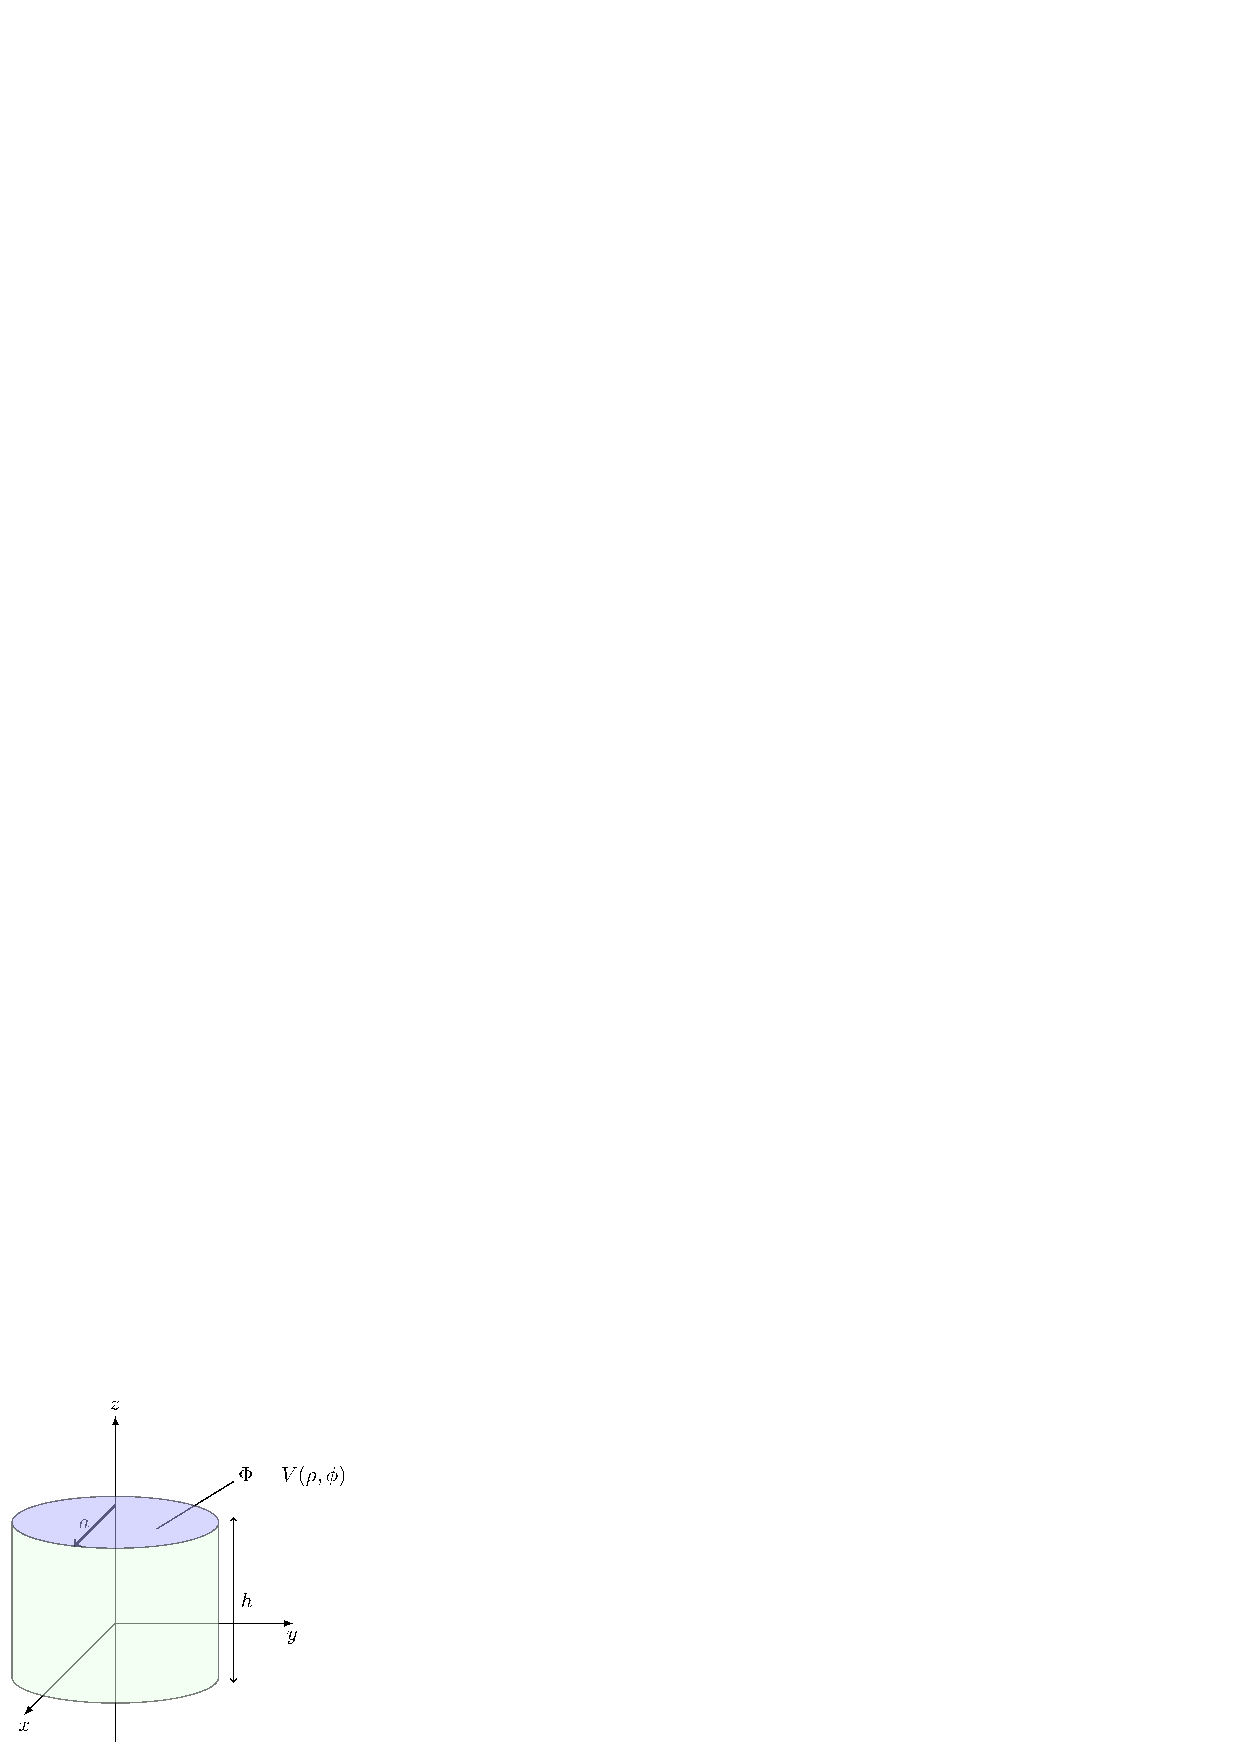
\includegraphics[scale=1]{Figuras/Cilindro_Bessel_01.pdf}
    \caption{Un cilindro conductor que tiene un potencial $V (\rho, \theta)$ en la tapa superior}%, mientras que el resto de la superficie está aterrizado.}
    \label{fig:figura_27_01}
\end{figure}
\end{frame}
\begin{frame}
\frametitle{Planteamiento del problema}
Supongamos que el potencial en la tapa superior varía como $V (\rho, \varphi)$ mientras que la superficie lateral y la tapa inferior están conectadas a tierra.
\end{frame}

\subsection{Resolviendo el problema}

\begin{frame}
\frametitle{Calculando el potencial}
Calculemos el potencial electrostático $\Phi$ en todos los puntos dentro del cilindro.
\end{frame}
\begin{frame}
\frametitle{Resolviendo el problema}
La solución general es el producto de las soluciones (\ref{eq:ecuacion_27_03}), (\ref{eq:ecuacion_27_04}) y (\ref{eq:ecuacion_27_13}):
\pause
\begin{align*}
\Phi (\rho, \varphi, z) = R(\rho) \, S(\varphi) \, Z(z)
\end{align*}
\end{frame}
\begin{frame}
\frametitle{La solución general}
Como $\Phi (\rho, \varphi, 0) = 0$ para cualquier valor arbitrario de $\rho$ y $\varphi$, \pause tenemos que $Z(0) = 0$, dando una constante $Z(z) = \sinh (l \, z)$.
\end{frame}
\begin{frame}
\frametitle{La solución general}
Ya que $\Phi (0, \varphi, z)$ es finito, \pause no se permite ninguna función de Neumann en la expansión y, dentro de una constante, tenemos $R (\rho) = J_{m}(l \, \rho)$.
\end{frame}
\begin{frame}
\frametitle{La solución general}
Además, como $\Phi (a, \varphi, z) = 0$ para cualquier valor arbitrario $\varphi$ y $z$, debemos de tener:
\pause
\begin{align*}
R (a) &= J_{m} (l \, a) = 0 \hspace{0.25cm} \Longrightarrow \hspace{0.25cm} l \, a = x_{mn} \\[0.5em]
&\Longrightarrow \hspace{0.25cm} l = \dfrac{x_{mn}}{a} \hspace{1cm} n = 1, 2, \ldots
\end{align*}
donde, $x_{mn}$ son las $n$-ésimas raíces de $J_{m}$.
\end{frame}
\begin{frame}
\frametitle{La solución general}
Ahora podemos multiplicar $R$, $S$ y $Z$ y luego sumar todos los valores posibles de $m$ y $n$, teniendo en cuenta que los valores negativos de $m$ dan términos que dependen linealmente de los valores positivos correspondientes.
\end{frame}

\subsection{Solución general}

\begin{frame}
\frametitle{La solución general}
El resultado es la llamada \textocolor{red}{serie de Fourier-Bessel}:
\begin{equation}
\begin{aligned}
\Phi (\rho, \varphi, z) &= \nsum_{m=0}^{\infty} \, \nsum_{n=1}^{\infty} J_{m} \left( \dfrac{x_{mn}}{a}  \, \rho \right) \, \sinh \left( \dfrac{x_{mn}}{a}  \, z \right) \times \\[1em]
&\times (A_{mn} \cos m \, \varphi + B_{mn} \sin m \, \varphi )
\end{aligned}
\label{eq:ecuacion_27_39}
\end{equation}
\end{frame}
\begin{frame}
\frametitle{La solución general}
Donde las constantes $A_{mn}$ y $B_{mn}$ deben ser determinadas por las CDF restantes que establecen que:
\pause $\Phi (\rho, \varphi, z) = V(\rho, \varphi)$ o:
\pause
\begin{equation}
\begin{aligned}
V (\rho, \varphi) &= \nsum_{m=0}^{\infty} \, \nsum_{n=1}^{\infty} J_{m} \left( \dfrac{x_{mn}}{a}  \, \rho \right) \, \sinh \left( \dfrac{x_{mn}}{a}  \, h \right) \times \\[1em]
&\times (A_{mn} \cos m \, \varphi + B_{mn} \sin m \, \varphi )
\end{aligned}
\label{eq:ecuacion_27_40}
\end{equation}
\end{frame}
\begin{frame}
\frametitle{Ajustando la expresión}
Multiplicando ambos lados por:
\pause
\begin{align*}
\rho \, J_{m} \left( \dfrac{x_{mk} \, a}{\rho} \right) \, \cos j \varphi
\end{align*}
\end{frame}
\begin{frame}
\frametitle{La solución general}
Para luego integrar de $0$ a $2 \, \pi$, y de $0$ a $a$ en $\rho$, se obtiene $A_{jk}$.
\\
\bigskip
\pause
Cambiando el coseno al seno, y siguiendo el mismo procedimiento, obtenemos $B_{jk}$.
\end{frame}
\begin{frame}
\frametitle{La solución general}
Regresamos del índice $m$ al $n$, por lo tanto:
\pause
\begin{align}
A_{mn} = \dfrac{\displaystyle 2 \scaleint{6ex}_{\bs 0}^{2 \pi} \! \dd{\varphi} \scaleint{6ex}_{\bs 0}^{a} \! \rho \, V (\rho, \varphi) \, J_{m} \! \left( \dfrac{x_{mn}}{a}  \, \rho \right) \, \cos m \varphi \dd{\rho}}{\pi \, a^{2} \, \left[ J_{m+1} (x_{mn}) \right]^{2} \, \sinh \left( \dfrac{x_{mn} \, h}{a} \right) }
\label{eq:ecuacion_27_41a}
\end{align}
\end{frame}
\begin{frame}
\frametitle{La solución general}  
\begin{align}
B_{mn} = \dfrac{\displaystyle 2 \scaleint{6ex}_{\bs 0}^{2 \pi} \! \dd{\varphi} \scaleint{6ex}_{\bs 0}^{a} \! \rho \, V (\rho, \varphi) \, J_{m} \! \left( \dfrac{x_{mn}}{a}  \, \rho \right) \, \sin m \varphi \dd{\rho}}{\pi \, a^{2} \, \left[ J_{m+1} (x_{mn}) \right]^{2} \, \sinh \left( \dfrac{x_{mn} \, h}{a} \right) }
\label{eq:ecuacion_27_41b}
\end{align}
en donde se ha utilizado la ec. (\ref{eq:ecuacion_27_24}).
\end{frame}

\subsection{De la simetría azimutal}

\begin{frame}
\frametitle{De la simetría azimutal}
El caso importante de simetría azimutal requiere una consideración especial.
\\
\bigskip
\pause
En tal caso, el potencial de la superficie superior $V (\rho, \varphi)$ debe ser independiente de $\varphi$.
\end{frame}
\begin{frame}
\frametitle{De la simetría azimutal}
Además, como $S (\varphi)$ es constante, su derivada debe anularse.
\\
\bigskip
\pause
Por lo tanto, la segunda ecuación en (\ref{eq:ecuacion_27_01b}) devuelve $\mu = -m^{2} = 0$.
\end{frame}
\begin{frame}
\frametitle{Expresión reducida}
Este valor cero de $m$ reduce la suma doble de la ec. (\ref{eq:ecuacion_27_39}) a una sola suma, y obtenemos:
\pause
\begin{equation}
\Phi (\rho, z) = \nsum_{n=1}^{\infty} A_{n} \, J_{0} \left( \dfrac{x_{0n}}{a}  \, \rho \right) \, \sinh \left( \dfrac{x_{0n}}{a}  \, z \right)
\label{eq:ecuacion_27_42}
\end{equation}
\end{frame}
\begin{frame}
\frametitle{Obteniendo los coeficientes}
Los coeficientes $A_{n}$ pueden obtenerse haciendo $m = 0$ en la primera ecuación de (\ref{eq:ecuacion_27_41a}):
\pause
\begin{equation}
A_{n} {=} \dfrac{4}{a^{2} \! \left[ J_{1} (x_{0n}) \right]^{2} \! \sinh \left( \dfrac{x_{0n} h}{a} \right)} \, \scaleint{6ex}_{\bs 0}^{a} \! \rho V (\rho) J_{0} \! \left( \dfrac{x_{0n}}{a} \! \rho \right) \! \dd{\rho}
\label{eq:ecuacion_27_43}
\end{equation}
donde $V(\rho)$ es el potencial independiente de $\varphi$ en la tapa superior del cilindro.
\end{frame}

% \subsection{Cilindro conductor con tapa a un potencial fijo $V_{0}$.}
% Supongamos que la tapa superior de un cilindro conductor se mantiene a un potencial constante $V_{0}$ mientras que la superficie lateral y la tapa inferior están conectadas a tierra.
% \par
% Queremos calcular el potencial electrostático $\Phi$ en todos los puntos dentro del cilindro.
% \par
% Como el potencial de la tapa superior es independiente de $\varphi$, prevalece la simetría azimutal y la ec. (\ref{eq:ecuacion_27_43}) nos devuelve
% \begin{align*}
% A_{n} &= \dfrac{4 \, V_{0}}{a^{2} \, J_{1}^{2} (x_{0n}) \, \sinh \left( \dfrac{x_{0n} \, h}{a} \right)} \, \scaleint{6ex}_{\bs 0}^{a} \rho \,  J_{0} \, \left( \dfrac{x_{0n}}{a}  \, \rho \right) \dd{\rho} \\[1em]
% &= \dfrac{4 \, V_{0}}{x_{0n} \, J_{1} (x_{0n}) \, \sinh \left( \dfrac{x_{0n} \, h}{a} \right)}
% \end{align*}
% donde hemos usado la ec. (\ref{eq:ecuacion_27_18}). El detalle del cálculo de la integral es \textbf{un problema a cuenta}. Se tiene entonces que
% \begin{align*}
% \Phi (\rho, z) = 4 \, V_{0} \, \nsum_{n=1}^{\infty} \dfrac{J_{0} \left( \dfrac{x_{0n} \, \rho}{a} \right) \, \sinh \left( \dfrac{x_{0n} \, z}{a} \right)}{{x_{0n} \, J_{1} (x_{0n}) \, \sinh \left( \dfrac{x_{0n} \, h}{a} \right)}}
% \end{align*}

\section{Problema con distribución de temperaturas}
\frame[allowframebreaks]{\frametitle{Temas a revisar} \tableofcontents[currentsection, hideothersubsections]}
\subsection{Geometría del problema}

\begin{frame}
\frametitle{Problema a resolver}
Se pide calcular la distribución de temperaturas dentro de un cilindro rígido.
\end{frame}
\begin{frame}
\frametitle{El problema con un cilindro}
Para iniciar bien la solución de cualquier ejercicio, conviene presentar un esquema del problema.
\\
\bigskip
\pause
En este caso, el cilindro rígido de radio $r = a$, como vemos en la siguiente figura:
\end{frame}
\begin{frame}
\frametitle{El problema con un cilindro}
\begin{figure}[H]
    \centering
    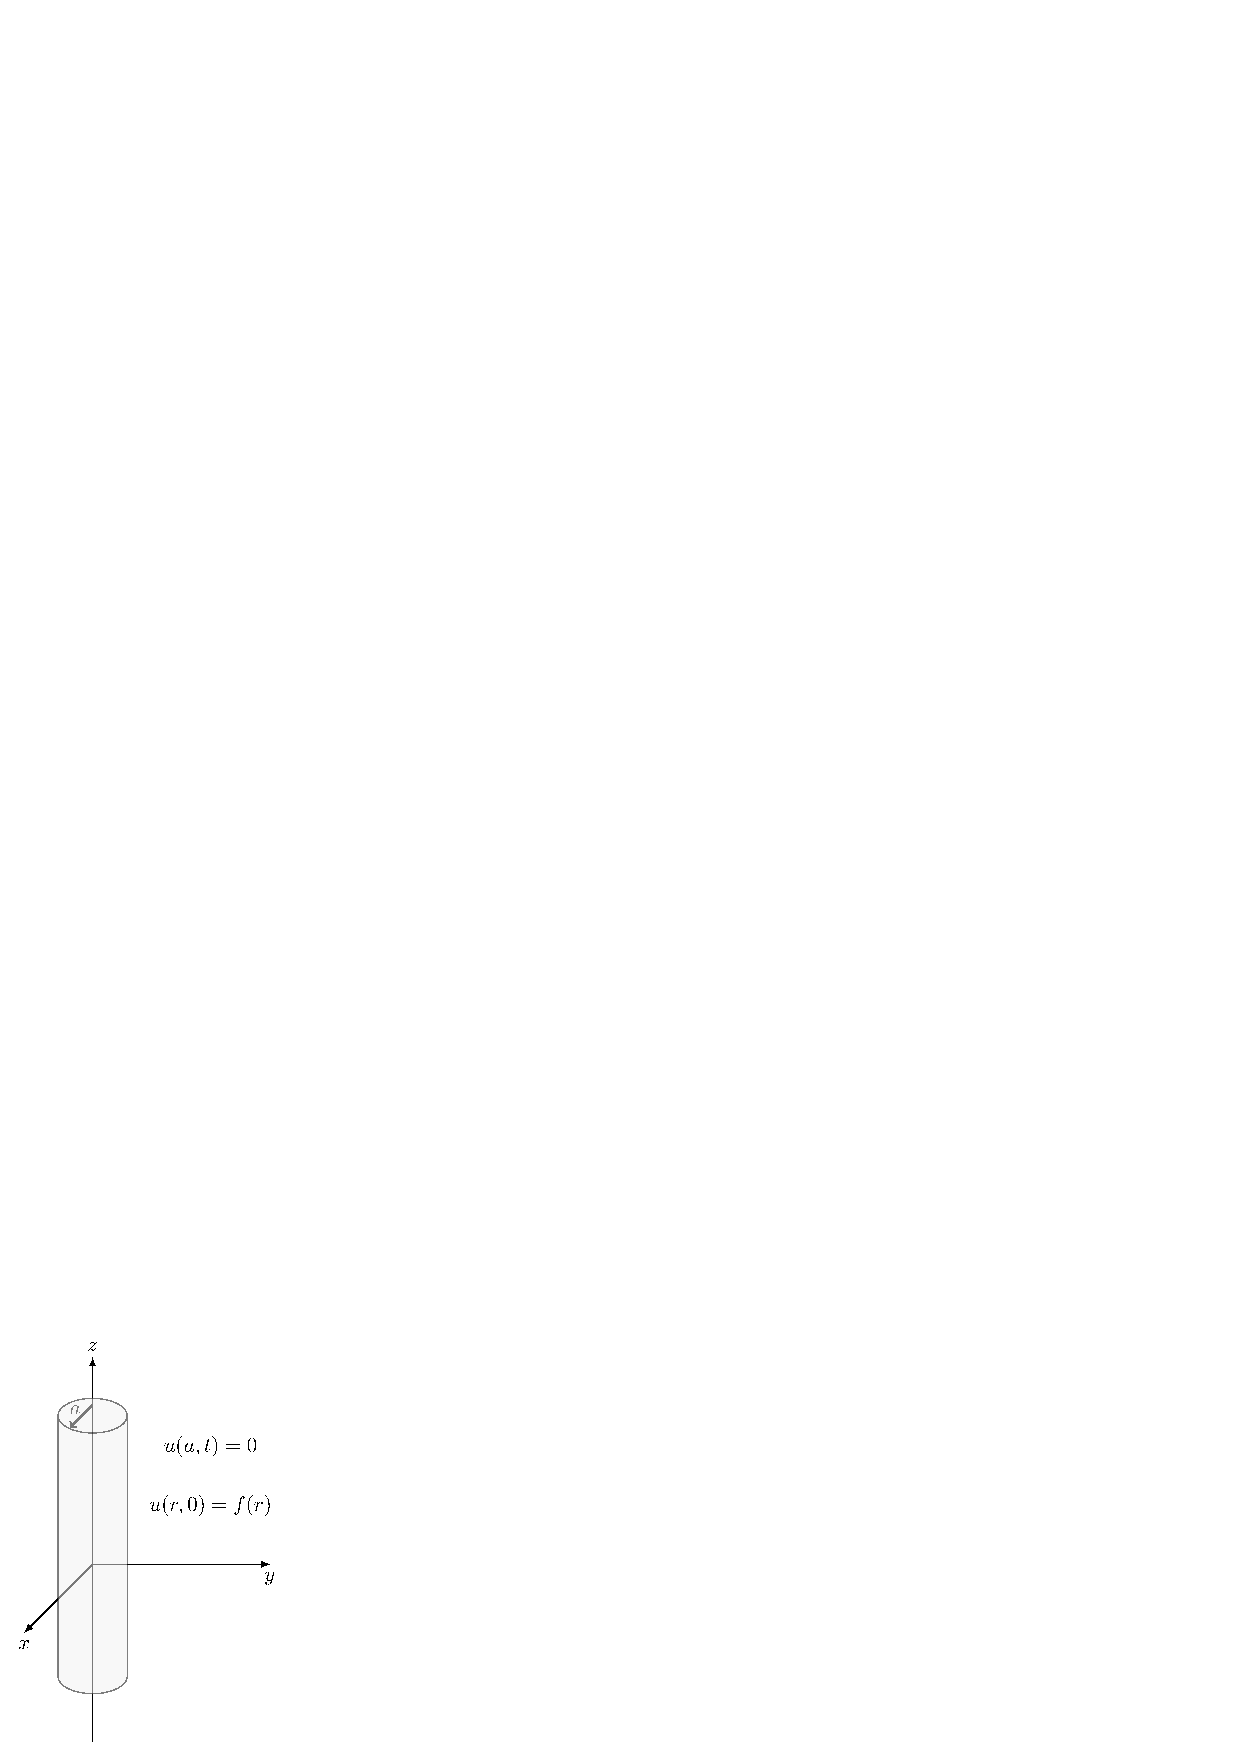
\includegraphics[scale=1]{Figuras/plot_cilindro_Bessel_01.pdf}
\end{figure}
\end{frame}
\begin{frame}
\frametitle{El problema con un cilindro}
Vemos que no importa la orientación del cilindro, ya sea que lo presentamos de manera horizontal o vertical, el punto importante es considerar que el eje $z$ \enquote{cruza} al cilindro por el centro.
\end{frame}

\subsection{Ecuación que modela el problema}

\begin{frame}
\frametitle{Ecuación a utilizar}
De acuerdo con lo que nos plantea el enunciado, la ecuación que debemos de ocupar, es la ecuación de calor:
\pause
\begin{align}
\pdv{u}{t} = \kappa \left( \pdv[2]{u}{r} + \dfrac{1}{r}  \, \pdv{u}{r} \right) \hspace{1cm} 0 < r < a, \hspace{0.5cm} t > 0
\label{eq:ecuacion_CilBessel_01}
\end{align}
\end{frame}
\begin{frame}
\frametitle{Condiciones del problema}
Junto con las condiciones:
\pause
\begin{align}
u (a, t) = 0 \hspace{2cm} u (r, 0) = f (r)
\label{eq:ecuacion_CilBessel_02}
\end{align}
Debemos de tomar en cuenta que la función $u (r, t)$ (solución) debe de ser acotada en todo el volumen del cilindro.
\end{frame}

\subsection{Resolviendo la ecuación}

\begin{frame}
\frametitle{Técnica de solución}
Tenemos una EDP lineal y homogénea, por lo que podemos apoyarnos con la técnica de \textocolor{cobalt}{separación de variables}.
\end{frame}
\begin{frame}
\frametitle{Aprovechando la simetría}
Como la distribución de temperatura no depende  de la parte angular $\theta$, así como del eje $z$, se simplifica el problema.
\end{frame}
\begin{frame}
\frametitle{Solución que se propone}
Se propone una solución del tipo:
\pause
\begin{align*}
u (r, t) = R (r) \, T (t)
\end{align*}
por lo que se calculan las derivadas parciales $u_{t}$, $u_{r}$ y $u_{rr}$, que vamos a sustituir en la ec. (\ref{eq:ecuacion_CilBessel_01}).
\end{frame}
\begin{frame}
\frametitle{Desarrollando la solución}
Se tiene entonces que:
\pause
\begin{align*}
u_{t} &= R (r) \, \pderivada{T} (t) \\[0.5em] 
u_{r} &= \pderivada{R} (r) \, {T} (t) \\[0.5em] 
u_{rr} &= \sderivada{R} (r) \, {T} (t)
\end{align*}
que se sustituyen en la ecuación de calor.
\end{frame}
\begin{frame}
\frametitle{Sustituyendo en la expresión}
Ocupando los valores de las derivadas, la ecuación tiene la forma:
\pause
\begin{align*}
R (r) \, \pderivada{T} (t) = \kappa \bigg[ \sderivada{R} (r) \, {T} (t) + \dfrac{1}{r} \, \pderivada{R} (r) \, {T}(t) \bigg]
\end{align*}
\end{frame}
\begin{frame}
\frametitle{Manejando la expresión}
Esta expresión la dividimos entre $R (r) \, T (t)$:
\pause
\begin{align*}
\dfrac{\pderivada{T}}{T} = \kappa \bigg[ \dfrac{\sderivada{R}}{R} + \dfrac{1}{r} \, \dfrac{\pderivada{R}}{R} \bigg]
\end{align*}
\end{frame}
\begin{frame}
\frametitle{Simplificando la expresión}
Simplificamos la expresión:
\pause
\begin{align*}
\dfrac{\sderivada{R} + \dfrac{1}{r} \pderivada{R}}{R} = \dfrac{1}{\kappa} \, \dfrac{\pderivada{T}}{T}
\end{align*}
\pause
Cada lado de la igualdad depende de una sola variable, al suponer que éstas son independientes entre sí, la única forma en la que se cumple la expresión, es que debe de ser igual a una constante.
\end{frame}
\begin{frame}
\frametitle{Constante de separación}
La constante de separación será: $-\lambda^{2}$. \pause La ecuación con la constante de separación es:
\pause
\begin{align*}
\dfrac{\sderivada{R} + \dfrac{1}{r} \pderivada{R}}{R} = \dfrac{1}{\kappa} \, \dfrac{\pderivada{T}}{T} = -\lambda^{2}
\end{align*}
\end{frame}
\begin{frame}
\frametitle{Usando las CDF}
Debemos de considerar la condición de frontera $u (a, t) = 0$:
\pause
\begin{align*}
R (a) \, T (t) = 0 \hspace{1cm} \Rightarrow \hspace{1cm} R (a) = 0
\end{align*}
\end{frame}
\begin{frame}
\frametitle{Sistema de EDO}
Llegamos a un sistema de dos EDO2H:
\pause
\begin{align}
\sderivada{R} (r) + \dfrac{1}{r} \, \pderivada{R} + \lambda^{2} \, R (r) &= 0, \hspace{1cm} R (a) = 0 \label{eq:ecuacion_CilBessel_03} \\[0.5em]  
\pderivada{T} (t) + \kappa \, \lambda^{2} \, T (t) &= 0 \label{eq:ecuacion_CilBessel_04}
\end{align}
\end{frame}

\subsection{La parte radial \texorpdfstring{$R (r)$}{R (r)}}

\begin{frame}
\frametitle{La parte radial de la ecuación}
La ec. (\ref{eq:ecuacion_CilBessel_03}) que es la parte radial del problema:
\pause
\begin{align*}
\sderivada{R} (r) + \dfrac{1}{r} \, \pderivada{R} + \lambda^{2} \, R (r) = 0
\end{align*}
\pause
es una ecuación de tipo Bessel:
\begin{align*}
\sderivada{y} + \dfrac{1}{x} \, \pderivada{y} + \left( \lambda^{2} - \dfrac{\nu^{2}}{x^{2}} \right) \, y = 0
\end{align*}
Con $\nu = 0$.
\end{frame}
\begin{frame}
\frametitle{Solución a la ec. tipo Bessel}
Sabemos que la solución general de la ED de Bessel de orden cero es de la forma:
\pause
\begin{align*}
R (r) = C_{1} \, J_{0} (\lambda \, r) + C_{2} \, Y_{0} (\lambda \, r)
\end{align*}
con las constantes $C_{1}$ y $C_{2}$ por determinar, $J_{0}$ es la función de Bessel de primer tipo, \pause mientras que $Y_{0}$ es la función de Bessel de segundo tipo (o funciones de Neumann).
\end{frame}

\subsection{Constricciones en el problema}

\begin{frame}
\frametitle{Usando las condiciones}
La función $R (r)$ debe de estar acotada en $r = 0$,  por lo que se deduce que $C_{2} = 0$, ya que:
\pause
\begin{align*}
Y_{0} (0) \to \infty
\end{align*}
\pause
Por lo tanto:
\begin{align*}
R (r) = C_{1} \, J_{0} (\lambda \, r)
\end{align*}
\end{frame}
\begin{frame}
\frametitle{Usando las condiciones}
Como $R (a) = 0$, tenemos:
\pause
\begin{align*}
C_{1} \, J_{0} (\lambda \, a) = 0
\end{align*}
\end{frame}
\begin{frame}
\frametitle{Usando las condiciones}
Se nos presentan dos casos:
\pause
\setbeamercolor{item projected}{bg=black,fg=white}
\setbeamertemplate{enumerate items}{%
\usebeamercolor[bg]{item projected}%
\raisebox{1.5pt}{\colorbox{bg}{\color{fg}\footnotesize\insertenumlabel}}%
}
\begin{enumerate}[<+->]
\item El caso trivial con $C_{1} = 0$.
\item El caso no trivial: $C_{1} \neq 0$, así:
\begin{align}
J_{0} (\lambda \, a) = 0
\label{eq:ecuacion_CilBessel_05}
\end{align}
\end{enumerate}
\end{frame}

\subsection{Soluciones a las EDO}

\begin{frame}
\frametitle{Soluciones a las ecuaciones}
Si $\lambda_{i} = 1, 2, \ldots$ son las raíces positivas (eigenvalores) de la ec. (\ref{eq:ecuacion_CilBessel_05}), se tiene que aparte del factor constante, las funciones:
\pause
\begin{align*}
R_{i} (r) = J_{0} (\lambda_{i} \, r) \hspace{1.5cm} i = 1, 2, \ldots
\end{align*}
son soluciones a la EDO2H radial, ec. (\ref{eq:ecuacion_CilBessel_03}), es decir, son las eigenfunciones.
\end{frame}
\begin{frame}
\frametitle{Soluciones a las ecuaciones}
Para los valores $\lambda$ considerados, la ec. (\ref{eq:ecuacion_CilBessel_04}), es decir, la parte temporal tiene las soluciones particulares:
\pause
\begin{align*}
T_{i} (t) = \exp(-\kappa \, \lambda_{i}^{2} \, t) \hspace{1.5cm} i = 1, 2, 3, \ldots
\end{align*}
\end{frame}
\begin{frame}
\frametitle{Soluciones a las ecuaciones}
La sucesión de funciones que son la solución completa:
\pause
\begin{align*}
u_{i} (r, t) = C_{i} \, J_{0} (\lambda_{i} \, r) \, \exp(-\kappa \, \lambda_{i}^{2} \, t) 
\end{align*}
satisfacen la ec. (\ref{eq:ecuacion_CilBessel_01}) así como la condición de frontera.
\end{frame}
\begin{frame}
\frametitle{Usando el principio de superposición}
De acuerdo con el principio de superposición, la función:
\pause
\begin{align}
u (r, t) = \nsum_{i=1}^{\infty} C_{i} \, J_{0} (\lambda_{i} \, r) \, \exp(-\kappa \, \lambda_{i}^{2} \, t)
\label{eq:ecuacion_CilBessel_06}
\end{align}
también satisface a la ecuación de calor inicial y la CDF.
\end{frame}
\begin{frame}
\frametitle{Usando el principio de superposición}
Ocupando la condición:
\pause
\begin{align*}
u (r, 0) = f (r)
\end{align*}
se obtiene la serie de Fourier-Bessel:
\pause
\begin{align}
f (r) = \nsum_{i=1}^{\infty} C_{i} \, J_{0}(\lambda_{i} \, r)
\label{eq:ecuacion_CilBessel_07}
\end{align}
quedando por determinar los coeficientes $C_{i}$.  %Para obtener esos coeficientes, haremos un breve repaso sobre las series de Fourier-Bessel.
\end{frame}

% \subsection{Series de Fourier-Bessel.}

% Supongamos que una función $f(x)$ tiene un desarrollo convergente de la forma:
% \begin{align}
% f (x) = \nsum_{i=1}^{\infty} C_{i} \, J_{\nu} (\lambda_{i} \, x) \hspace{1cm} 0 < x < a
% \label{eq:ecuacion_CilBessel_08}
% \end{align}
% donde los $\lambda_{i}$ con $i = 1, 2, \ldots$ son las raíces positivas de $J_{\nu} (\lambda \, a) = 0$. Multiplicamos ambos lados de la ec. (\ref{eq:ecuacion_CilBessel_08}) por $x \, J_{\nu}(\lambda_{j} \, x)$ con $j$ fijo, para luego integrar entre $0$ y $a$, suponiendo que la serie es integrable término a término, llegando a:
% \begin{align*}
% \scaleint{6ex}_{\bs 0}^{a} &x \, f(x) J_{\nu}(\lambda_{j} x) \dd{x} = \\[0.5em]
% &= \nsum_{i=1}^{\infty} C_{i} \scaleint{6ex}_{\bs 0}^{a} x \, J_{\nu} (\lambda_{i} x) \, J_{\nu} (\lambda_{j} x) \dd{x}
% \end{align*}
% Para resolver la integral del lado derecho:
% \begin{align*}
% \scaleint{6ex}_{\bs 0}^{a} x \, J_{\nu} (\lambda_{i} x) \, J_{\nu} (\lambda_{j} x) \dd{x}
% \end{align*}
% habrá que emplear la propiedad de ortogonalidad de las funciones de Bessel. Sabemos que las funciones de Bessel cuentan con la propiedad de ortogonalidad, dada por la expresión:
% \begin{align*}
% \scaleint{5ex}_{\bs 0}^{a} &x \, J_{\nu} (\lambda_{i} \, x) \, J_{\nu} (\lambda_{j} \, x) \dd{x} = \\[1em]
% &= \begin{cases}
% 0 & i \neq j \\
% \dfrac{a^{2}}{2} \, \big[ J_{\nu+1} (\lambda_{i} \, a)\big]^{2} & i = j, \hspace{0.5cm} i = 1, 2, \ldots
% \end{cases}
% \end{align*}
% Los coeficientes $C_{i}$ son entonces:
% \begin{eqnarray*}
% \begin{aligned}
% C_{i} &= \dfrac{\scaleint{5ex}_{\bs 0}^{a} x \, f(x) \, J_{\nu}(\lambda_{i} \, x) \dd{x}}{\scaleint{5ex}_{\bs 0}^{a} x \, \big[ J_{\nu} (\lambda_{i} \, x) \big]^{2} \dd{x}} \hspace{1cm} i = 1, 2, \ldots \\[1em] 
% &= \dfrac{\scaleint{5ex}_{\bs 0}^{a} x \, f(x) \, J_{\nu}(\lambda_{i} \, x) \dd{x}}{\dfrac{a^{2}}{2} \, \big[ J_{\nu+1} (\lambda_{i} \, a) \big]^{2}} \hspace{1cm} i = 1, 2, \ldots
% \end{aligned}
% \end{eqnarray*}
% Por lo tanto, los coeficientes $C_{i}$ quedan definidos por la expresión:
% \begin{align*}
% C_{i} = \dfrac{2}{a^{2}} \dfrac{\scaleint{5ex}_{\bs 0}^{a} x \, f(x) \, J_{\nu}(\lambda_{i} \, x) \dd{x}}{ \big[ J_{\nu+1} (\lambda_{i} \, a) \big]^{2}} \hspace{1cm} i = 1, 2, \ldots
% \end{align*}
% Con este resultado, ya podemos regresar al ejercicio y definir la solución completa al problema.

% \subsection{Regresando a la solución.}

\subsection{Los coeficientes}

\begin{frame}
\frametitle{Los coeficientes determinados}
Con acuerdo a la manera en que se obtuvieron los coeficientes $C_{i}$ de una serie de Fourier-Bessel, para el problema del cilindro, se tiene que:
\pause
\begin{align}
\begin{aligned}
C_{i} = \dfrac{2}{a^{2} \, \big[ J_{1} (\lambda_{i} \, a) \big]^{2}} &\scaleint{6ex}_{\bs 0}^{a} r \, f(r) \, J_{0}(\lambda_{i} \, r) \dd{r} \\[0.5em]
i &= 1, 2, \ldots
\end{aligned}
\label{eq:ecuacion_Cil_Bessel_09}
\end{align}
\end{frame}
\begin{frame}
\frametitle{Distribución de temperaturas}
La distribución de temperaturas en el cilindro viene dada por la expresión:
\pause
\begin{eqnarray}
\begin{aligned}[b]
u (r, t) &= \dfrac{2}{a^{2}} \nsum_{i=1}^{\infty} \bigg[ \, \scaleint{6ex}_{\bs 0}^{a} \, r \, f(r) J_{0} (\lambda_{i} \, r) \dd{r} \bigg] \times \\[1em]
&\times \dfrac{J_{0} (\lambda_{i} \, r)}{\big[ J_{1} (\lambda_{i} \, a) \big]^{2}} \, \exp( -\kappa \, \lambda_{i}^{2} \, t)
\end{aligned}
\label{eq:ecuacion_CilBessel10}
\end{eqnarray}
donde la suma es tomada sobre todas las raíces positivas de la ec. (\ref{eq:ecuacion_CilBessel_05}).
\end{frame}

\section{Ejercicios a cuenta}
\frame[allowframebreaks]{\frametitle{Temas a revisar} \tableofcontents[currentsection, hideothersubsections]}
\subsection{Enunciados}

\begin{frame}
\frametitle{Ejercicio 1}
%Referencia Hassani - Chapter 12
Un cilindro largo conductor de calor de radio $a$ se compone de dos mitades (con secciones transversales semicirculares) con un espacio infinitesimal entre ellas.
\\
\bigskip
\pause
Las mitades superior e inferior del cilindro están en contacto con baños térmicos $+T_{0}$ y $-T_{0}$, respectivamente. Encuentra la temperatura tanto dentro como fuera del cilindro.
\end{frame}
\begin{frame}
\frametitle{Ejercicio 2}
%Referencia Hassani - Chapter 12
Un cilindro largo conductor de calor de radio $a$ se compone de dos mitades (con secciones transversales semicirculares) con un espacio infinitesimal entre ellas.
\\
\bigskip
Las mitades superior e inferior del cilindro están en contacto con baños térmicos $+T_{1}$ y $-T_{1}$, respectivamente.
\end{frame}
\begin{frame}
\frametitle{Ejercicio 2}
El cilindro está dentro de otro cilindro de radio $b$ más grande ( $a < b$ y coaxial con él) que se mantiene a la temperatura $T_{2}$.
\\
\bigskip
\pause
Encuentra la temperatura dentro del cilindro interno, entre los dos cilindros y fuera del cilindro externo.
\end{frame}

\end{document}